\documentclass[conference]{IEEEtran}
\IEEEoverridecommandlockouts
% The preceding line is only needed to identify funding in the first footnote. If that is unneeded, please comment it out.
\usepackage{cite}
\usepackage{url}
\usepackage{amsmath,amssymb,amsfonts}
%\usepackage{algorithmic}
\usepackage{graphicx}
\usepackage{textcomp}
\usepackage{xcolor}
\usepackage{svg}
\usepackage{tabularx}
% \usepackage{algorithm}
\usepackage{algpseudocode}
\usepackage{subfig}
\DeclareMathOperator{\atantwo}{atan2}
\newcommand{\mywhile}{\textbf{while}}
\newcommand{\myendwhile}{\textbf{end while}}
\usepackage{siunitx}
\usepackage[hidelinks]{hyperref}
\usepackage{caption}
\usepackage{subcaption}
\renewcommand{\labelenumi}{}
\def\BibTeX{{\rm B\kern-.05em{\sc i\kern-.025em b}\kern-.08em
    T\kern-.1667em\lower.7ex\hbox{E}\kern-.125emX}}
\usepackage{lscape}
\begin{document}

\title{Localization, collision avoidance, and centroid navigation of parachutes swarm}

\author{
\IEEEauthorblockN{Niccolò Andreetta}
\IEEEauthorblockA{niccolo.andreetta@studenti.unitn.it\\
M.N. 232077}
\and
\IEEEauthorblockN{Simone Manfredi}
\IEEEauthorblockA{simone.manfredi@studenti.unitn.it\\
M.N. 239337}
}

\maketitle

\begin{abstract}
This project deals with the localization and control of a swarm of parachutes intended to be dropped from a certain height and autonomously reach a desired location on the ground. In particular, each agent controls its movement to drive the centroid of the storm towards the desired final location.\\
The parachutes are firstly modelled as devices able to move independently along the three cartesian axes (thanks to an actuator in each of them), while later, they are modelled as unicycles with forward velocity, rotation and falling velocity controls. \\
The main features that each parachute has to implement are self-localization in the space (via absolute and relative position measurement), the optimal control to design the trajectory to be followed, and collision avoidance.\\
The simulation results show that the parachutes can accomplish their task and reach the ground without any collision, even in the presence of noises in the inputs, dynamics and GPS tracking.
\end{abstract}
\section{Introduction}
The fields of distributed systems and optimal control play an essential role in modern problems, such as precision-guided parachutes for cargo delivery \cite{b2} \cite{b3}.\\
This project aims to drive the centroid of a storm of falling parachutes from the initial releasing point to the desired landing target on the ground. To pursue this purpose, each agent must always be able to identify the geometric centroid of the storm and move such that the new mean point position accomplishes what the motion trajectory planner defines. It must be noted that here, the focus is on the mean point of the formation so that the single parachutes can land in the neighbourhoods of the arrival location.\\
Along with the distribution of information and path control, collision avoidance is a critical requirement because any crash can lead to an uncontrolled fall of the agents.\\
The available hardware to each parachute is composed of some measurement systems allowing the localization in space, the communication between each other, and the measurement of relative distances.\\
The limitations of the scope of this project are the following: the dynamic of the parachutes is simplified, the actuators have not been practically identified, two parachutes in the storm can either communicate with one another or cannot communicate at all (i.e. unidirectional communication is not taken into account).
\section{Adopted models}
\subsection{Simplified parachute model}
The considered parachutes are made of two main parts: a sail with finite radial dimensions and height and a payload with dimension negligible compared to the first. The latter is placed below the former and carries also the communication, measurement and control systems.\\
The most simple dynamical parachute model is linear and considers three actuators able to move the device in space, while gravity acts as non-controllable input along the vertical direction.
% Matrix expression placed in another file for clarity
\begin{gather}
\label{eq:model_1}
    x_{i+1} = Ax_i + Bu + G\nu \\
    \begin{bmatrix}
    x_{i+1}\\
    y_{i+1}\\
    z_{i+1}
    \end{bmatrix}=
    %\begin{bmatrix}
    I_3
    %\end{bmatrix}
    \begin{bmatrix}
    x_{i}\\
    y_{i}\\
    z_{i}
    \end{bmatrix} +
    \Delta t
    %\begin{bmatrix}
    I_3
    %\end{bmatrix}
    \begin{bmatrix}
    v_x\\
    v_y\\
    v_z
    \end{bmatrix} + %\notag \\
    \begin{bmatrix}
    1&0&0&0\\
    0&1&0&0\\
    0&0&1&\Delta t
    \end{bmatrix}
    \begin{bmatrix}
    \nu_x\\
    \nu_y\\
    \nu_z\\
    \bar{v_z}
    \end{bmatrix}
     \notag
\end{gather}
The uncertainties $\nu_x$, $\nu_y$, and $\nu_z$ model the wind disturbances and the error along the three directions ($\left[\nu_x \, \nu_y \,\nu_z \right]\sim\mathcal{N}\left(0_3, L\right)$), while $\bar{v_z}$ is the velocity at which the parachutes fall due to the gravity action. 

$\bar{v_z}$  is the non-controllable input related to the gravity that pulls the parachute to the ground.\\
In this way, the total velocity in the z direction has been split into a non-controllable part, which is the one related to gravity, and into a controllable one. A parachute can reduce its falling velocity by breaking until a minimum one (necessary to avoid the closure of the sail) or accelerate up to the maximum one given by its geometry.\\
Following typical values for these physical parameters, for the simulation it has been chosen to set the maximum free-falling speed to 55 $\left[\si{\meter\per\second}\right]$ \cite{b8}, and a maximum falling one when the parachute is opened equal to 4.87 $\left[\si{\meter\per\second}\right]$, considering a mass of 100 $\left[\si{\kilogram}\right]$, a drag coefficient of 1.5 and a parachute's area of 45 $\left[\si{\meter^2}\right]$,  $\bar{v}_{z,max} = \sqrt{\frac{2 \, m \, g}{c_p \, \rho \, A}} = 4.87 \left[\si{\meter\per\second}\right]$ \cite{b9}. \\
Regarding the minimum falling velocity, a value equal to 25\% of the maximum one has been selected arbitrarily because it is hard to define without real experiments.\\
Even though a physical system able to provide the required displacement on the plane has not been identified, some minimal performances in movement and errors in the actuation have been considered.

\subsection{Unicycle-like parachute model} \label{unicyle}
A more sophisticated analysis can consider that a real parachute can brake the fall and steer by toggling the lines connecting the sail and the payload. At the same time, it has only a forward velocity. These considerations suggest that it can be modelled as a unicycle, with equations given by (\ref{eq:NL}).
\begin{equation}
\label{eq:NL}
    \begin{gathered}
       x_{i+1} = x_i + V\cos{\theta}\Delta t + \nu_x  \\
       y_{i+1} = y_i + V\sin{\theta}\Delta t  + \nu_y\\ 
       z_{i+1} = z_i + \bar{v_z}\Delta t + v_z\Delta t + \nu_z\\ 
       \theta_{i+1} = \theta_i + \omega\Delta t + \nu_{\theta} 
    \end{gathered}
\end{equation}
Hence, the control inputs are the forward and the rotational velocity and the falling breaks, named $V$, $\omega$, and $v_z$.
Even though in a real parachute, a minimum forward velocity is necessary to ensure the lift force sustaining the fly, in this project, the forward velocity has been assumed to be bounded between 0 and a maximum value to simplify the control laws.\\
For what concerns the boundaries of the inputs, a maximum forward velocity of 13 $\left[\si{\meter\per\second}\right]$ has been selected \cite{b7} \cite{b10}, while the maximum rotation speed is 0.52 $\left[\si{\radian\per\second}\right]$. As for the control in the vertical direction, the same holds from the linear model.

\subsection{Communication system}\label{communication}
The adopted communication system has to allow bidirectional data exchange between chutes moving in the space. For example, this can be achieved by using a UWB mounted on the payload, which has a typical communication range of 50 $\left[\si{\meter}\right]$ \cite{b11}.\\
The measurement of the absolute position is done using a GPS, with an uncertainty of 5 $\left[\si{\meter}\right]$ while for what concerns the relative measurement, multiple technologies can be used such as LIDAR, stereo camera or the combination of a UWB and a camera. For the seek of the thesis, it is assumed that the relative measurement can be done when the agents are closer than 50 $\left[\si{\meter}\right]$ and are provided with an uncertainty of 1 $\left[\si{\meter}\right]$. It is also assumed that each agent can measure its orientation with respect to a fixed direction but cannot measure the others'.
\section{Solution}\label{sec:solution}
\subsection{Localization}\label{subsec:solution_localization}
For the localization, a Kalman Filter (KF) or Extended Kalman Filter (EKF) \cite{b12} (according to the considered dynamic) and a distributed Weighted Least Square (WLS) has been used. In particular, each agent localizes itself running a KF/EKF that updates its prediction with only an absolute measurement (i.e. from the GPS). In a following step, each agent measures the relative distance from the others and then project them back in the world reference frame (i.e. a frame common for all the parachutes). Finally, the network runs a distributed WLS in order to share the knowledge with the team in a distributed way. The KF/EKF works as optimal filter under the hypothesis that the noise acting on the system is white, gaussian with zero mean, \textcolor{blue}{and uncorrelated from the one acting on the measurement}, the sensors are calibrated and affected by a zero mean white noise.\\
 To ensure the reaching of the average consensus the transition matrix describing the system at each time step has to be doubly stochastic, implying that the communication between agents has to be bidirectional.\\
 \textcolor{blue}{The distribution of the localization has been done applying the distribute WLS algorithm presented in the course \cite{b13}. In particular, each agent \textit{i} able to communicate with another shares its own localization and the one done on the others \textit{j} in the swarm, alongside with the associated covariance matrices. The assumption on which the algorithm is based is that the localization done by \textit{i} on agent \textit{$j_1$} is uncorrelated on the one done on \textit{$j_2$}, which implies that the covariance matrix (called C in \cite{b13}) build during the consensus is block diagonal (even though each block is not necessarily diagonal). The Metropolis-Hastings time-varying weighting scheme.\\
The result of the consensus is that each agent may have improved the localization on other that haev already seen, but also fo some furthert that were not directly measured before, and for which the information come with message exchange.}. Note that now, the self-localization of agent \textit{i} now depends also on the self localization of the others (which is embedded in the relative measurement). This implies that agent \textit{i} cannot use the output of the consensus as input of the new round of KF/EKF, because \textcolor{blue}{KFs/EKFs} cannot be used in cascade. For this reason, before running another round of localization, each agent discards the information of its position reached with the WLS and so the \textit{previous} at KF/EKF step k+1 is the output of step k. This is done to ensure that the input of a KF is uncorrelated from the output of the others.\\
In the picture, a probability of performing the GPS and the relative distance measurement are taken into account.

\subsection{Collision avoidance}
After having localized each agent, the collision avoidance is necessary to let each robot be reasonably further from the others in order to not get tangled when moving in the space. This requirement has also to be fulfilled while the agents are moving in a 3D environment, taking into account a finite size of the parachutes, the knowledge of the position of only a subset of agents (furthermore with a certain level of uncertainty). All these features may be well obtained dividing the working space with a Voronoi tessellation and enforcing each agent to move remaining inside its own cell. \\
The basic idea behind the tessellation is to assign to an agent \textit{i} all the points of the mission space $q \in \mathcal{Q} \subseteq \mathbb{R}^2$ closer to it more than to the others agents \textit{j} \cite{b1}:
\begin{equation}
    \mathcal{V}_i = \left\{ q \in \mathcal{Q} \lvert \left\lVert q-p_i \right\rVert \leq \left\lVert q-\hat{p_j} \right\rVert, \forall j \neq i, j \in \tilde{\mathcal{N}_{i}} \right\}
\end{equation}
where $p_i=\left[x_i, y_i\right]^T$ is the location of the agent \textit{i} while $\hat{p_j}$ is the one of agent \textit{j} (eventually properly projected in order to achieve some further features, as will be explained in \autoref{sec:implementation_details}).\\
The decentralization of the algorithm implies that each agent performs the tessellation of only a surrounding area of radius $R_s$, called \textit{sensing range} which is usually set at $R_s = R_c/2$, with $R_c$ the furthest distance from where an agent can measure the position of another, called \textit{communication range}. The \textit{neighbour set} $\tilde{\mathcal{N}_{i}}$ is composed by all the egents for which the position is known either by consensus or direct measure. \\
During the navigation, the entity used to represent the agent is its centroid, and so all the computations are done in order to ensure that this specific point remains inside the designed area. The finite dimension of the agent $\delta_i$ has to be taken into account because otherwise the parachute may exceed the prescribed limit even tough its centroid remains inside the cell. In order to avoid this, the dimension of the tessellation has to be shrunk such that when the centre of the agent reaches the new edge, its encumbrance arrives at the old limit. Furthermore, since the algorithm is implemented in discrete time, then the evolution of the system between one time instant and the following has to be considered beforehand, assuming that the agent may always move of the maximum amount allowed by the actuators in one time step.\\
\textcolor{blue}{Given that} the environment where the parachutes fly is a 3D space, then in principle the voronoi tessellation have to be expanded at the whole volume of movement. However, the problem can be still seen as a planar one by projecting the location of the surrounding agents in the plane of the one doing the tessellation when these are reasonably close to each others. Furthermore, in the case that the chute admits an actuation in the vertical direction, then the tessellation concept can be extended in the vertical axis in order to ensure the collision avoidance even in that dimension. Here the safe space is the one between the agents itself and a minimum height called $z_{min}$.
\subsection{High-level motion control}
\textcolor{blue}{The high-level motion control deals with the problem of how and where to move the centroid, in order to make it land on the target. Furthermore, since the centroid is a function of the single parachute location, it coordinates the agetns' movements in order to realized the prescribed centroid trajectory. The actuators command enabling this displacement are instead sintetized by the \textit{low-level controller}.}\\
In this work, the centroid is modeled as a fictional fully actuated robot with a linear dynamic in 2 dimensions, as shown in (\ref{robot}): since the target position is on the ground, the convergence in the z direction is guaranteed by the action of gravity, so the actuators must only work in the $xy$ plane.\\
\begin{equation}
    \begin{bmatrix}
        x_{i+1}\\
        y_{i+1}
    \end{bmatrix}=
    \begin{bmatrix}
        I_2
    \end{bmatrix}
    \begin{bmatrix}
        x_i\\
        y_i
    \end{bmatrix}
    +\Delta t\begin{bmatrix}
        I_2
    \end{bmatrix}
    \begin{bmatrix}
        v_{x,i}\\
        v_{y,i}
    \end{bmatrix}
    \label{robot}
\end{equation}
An LQR algorithm \cite{} has been used to find the optimal input $u$ to be fed to the \textcolor{blue}{fake agent}. This algorithm can only be used for linear systems and it finds the global optimum of the problem, which is calculated by means of a minimization of a cost function, expressed as:
\begin{equation}
    J = \sum_{k=t}^{N-1} x_k^TSx_k + u_k^TRu_k
\end{equation}
where $S$ and $R$ are the state and input cost matrices, which can be modeled to improve the state or the input minimization, and $x$ and $u$ are the actual state and input.\\
In the discrete time, finite horizon domain, the optimum input is given by:
\begin{equation}
    u_t=K_tx_t 
\end{equation}
where $K_t$ is the optimal gain matrix given by the algorithm.\\
Once the optimal control for the fictional robot is found, following the kinematics shown in the equations (\ref{robot}), its next desired position is calculated.\\
The computation of the desired position of each parachute that realize the desired movement of the global centroid is not trivial. In fact, the global centroid is a function of each parachute position, and the inverse kinematic (i.e. finding the parachutes' positions that realize a desired position in the centroid) is over-determined. \textcolor{blue}{Two solutions has been proposed to solve this problem, while a third one to be used is used in some \textit{emergency} situations to avoid collision will be presented in \autoref{sec:details_high_level}, after the motivations why it is necessary.
\subsubsection{Same control for all the chutes}
 A quick and intuitive but "forced" solution consists of feeding in the parachutes the exact same control input found in the LQR problem since if every parachute moves in the same way then the global centroid will be moved accordingly.
 \subsubsection{Inverse kinematics}
  A more robust solution comes from comparing this problem to the well-known and solved problem of redendancy in robotics. In fact, as in overactuated manipulators there are infinite joints' position realizing a desired end effector position, here infinite agents' positoin realize the centroid one. However, a numerical approach has been developed in the past years to solve inverse kinematics by a \textit{postural task}, which is just an arbitrary chosen secondary task in the joint space that does not affect the motion of the end-effector  but identifies one solution among the infinite ones \cite{b5} \cite{b6}.\\
In this specific case two possible secondary tasks may be to let each single agent converge toward the land target or toward the global centroid. The algorithm can give more priority to pricipal or secondary requirement  according to a weighting value that can be chosen arbitrary.}

\subsection{Low-level motion control}
Given the single parachute target point from the high-level control, the goal of the low level control is to provide the input that ensures to move towards it while not exceed the motion boundaries identified by the Voronoi tessellation. 
\subsubsection{Control of linear model}
In case of linear dynamics, one possible control law is the one proposed by \cite{b1}:
\begin{gather}
    \label{eq:proportional}
    u=-k_p\left(p_i - C_{\mathcal{V}_i}\right)\\
    \label{centroid}
    C_{\mathcal{V}_i} = \frac{1}{M_{\mathcal{V}_i}}\int_{\mathcal{V}_i}\varphi\left(q\right)qdq \text{ , } M_{\mathcal{V}_i} = \int_{\mathcal{V}_i}\varphi\left(q\right)dq
\end{gather}
with, for the planar motion, $\varphi\left(q\right)$ is a bivariate pdf centred in the point identified by the high level control. \textcolor{blue}{This controrl law uses the property that each point inside the voronoi cell can be reached by the agent with a staright motion}.\\
For what concerns the control on the vertical axis, as said before the velocity input has to be constrained. In particular, a proportional gain has been chosen to break when the $z_{min}$ is near to the parachute:
\begin{equation}
\label{control_law_z}
    \begin{gathered}
        k_{pz}=-\bar{v}_z/R_{sv}\\
        u_{tmp}=-\bar{v}_z-k_{pz}(z_i-z_{min,i})\\
        v_z=\min(u_{tmp}, v_{z,min}-\bar{v}_z)
    \end{gathered}
\end{equation}
In this way, when there is non parachute under the agent $i$, $(z_i-z_{min,i})=R_{sv}$ and so the control $v_z$ is zero, meaning that there is no need to break. On the other hand, when $(z_i-z_{min,i})=0$, meaning that the parachute would not want to go down because the other agents is too near, the input is $v_{z,min}-\bar{v}_z$, such that when in the dynamics it is added the effect of gravity (\ref{eq:model_1},\ref{eq:NL}) the sum results in the minimum vertical velocity: the agent cannot stop in the air but has to descent with some velocity.\\
The physical actuation in z opens or closes the sails, meaning that it changes the the $\beta$ coefficient in (\ref{eq:drag_force}) and so the free falling velocity. It has been decided to considered $\beta$ as constant and we have directly modified the velocity.\\
\textcolor{blue}{Since the external disturbances act directly on the positions, then the effective velocities can be locally grater or smaller than the boundaries.}
\subsubsection{Contorl of the unicycle model}
\textcolor{blue}{Since the trajectory followed by the nonlinear agents may exceed the voronoi cell limits with the afermentioned control law, a more complex one has to be used. In this work, the control law (\ref{eq:control_law}), proposed by \cite{b4} is allows to guarantee the convergence of the parachute towards the target in a fast and elegant way (without the use of a PID controller), and also to find the so called \textit{Feedback Motion Predict}, which is the area that can be occupied by the parachute during the execution of the control law (\ref{eq:control_law}).}
\begin{equation}
\label{eq:control_law}
    \begin{gathered}
        v_y = k_v\max\Big(0,\begin{bmatrix}
           \cos{\theta} & \sin{\theta}
       \end{bmatrix}(C_{\mathcal{V}_i} -p_i)\Big)\\
        \omega = k_{\omega}\atantwo\Big(\begin{bmatrix}
           -\sin{\theta} \\ \cos{\theta}
       \end{bmatrix}^T(C_{\mathcal{V}_i} -p_i),\begin{bmatrix}
           \cos{\theta} \\ \sin{\theta}
       \end{bmatrix}^T(C_{\mathcal{V}_i} -p_i)\Big)
    \end{gathered}
\end{equation}
\begin{figure}[t]
    \centering
    \subfloat[][\emph{Truncated Ice-Cream Motion Cone updating as the agent moves.}]{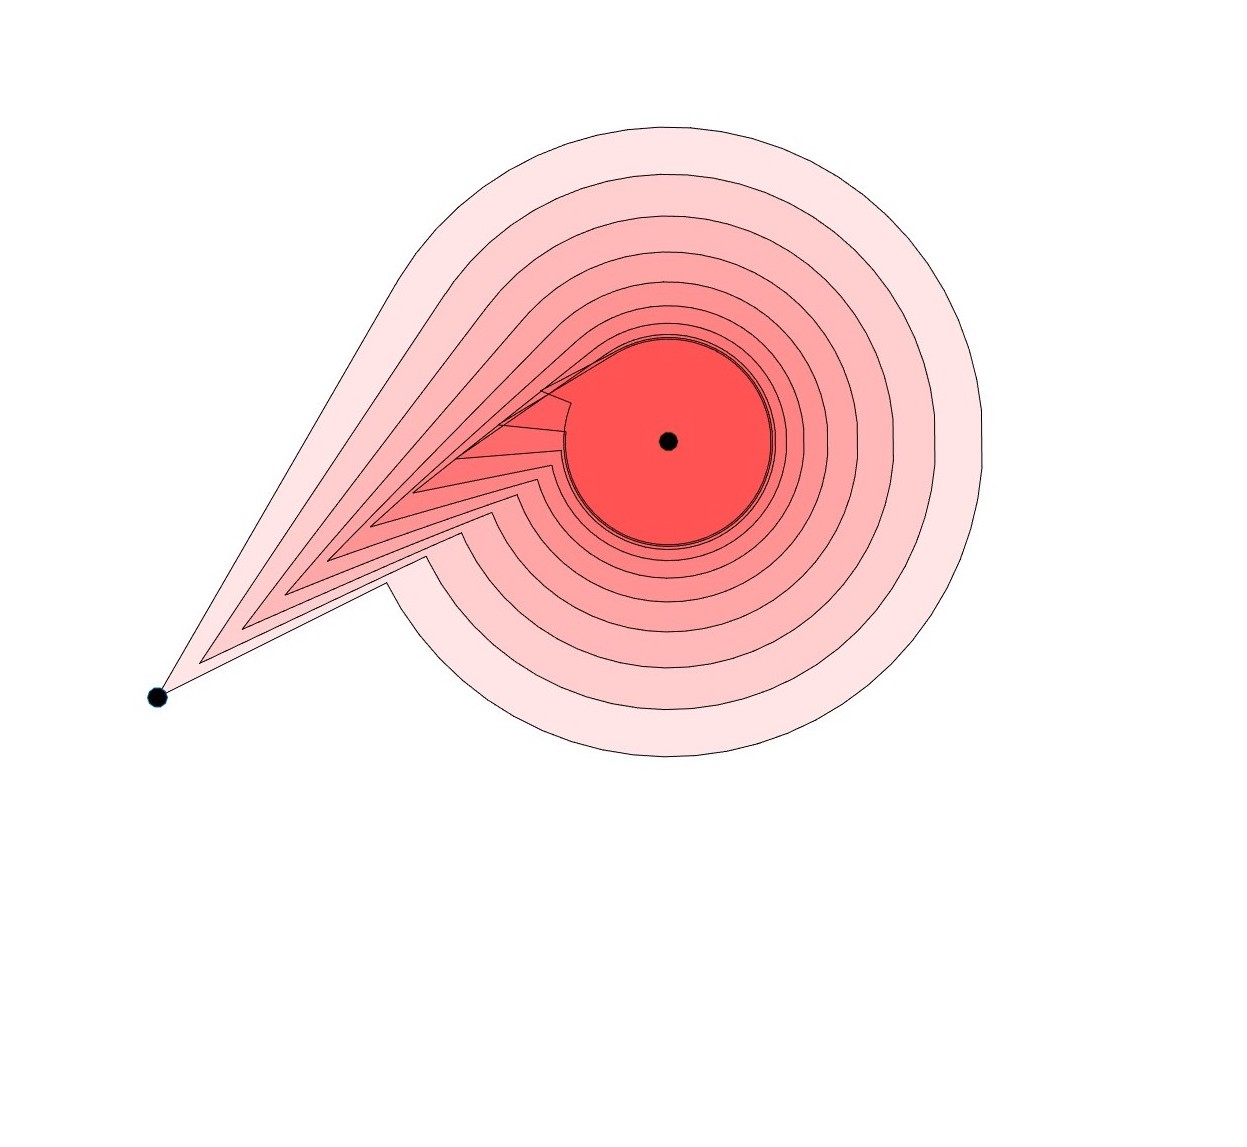
\includegraphics[scale=.08]{images/cone.jpg}} \quad
    \subfloat[][\emph{The cone is moved to be fit into the Voronoi cell.}]{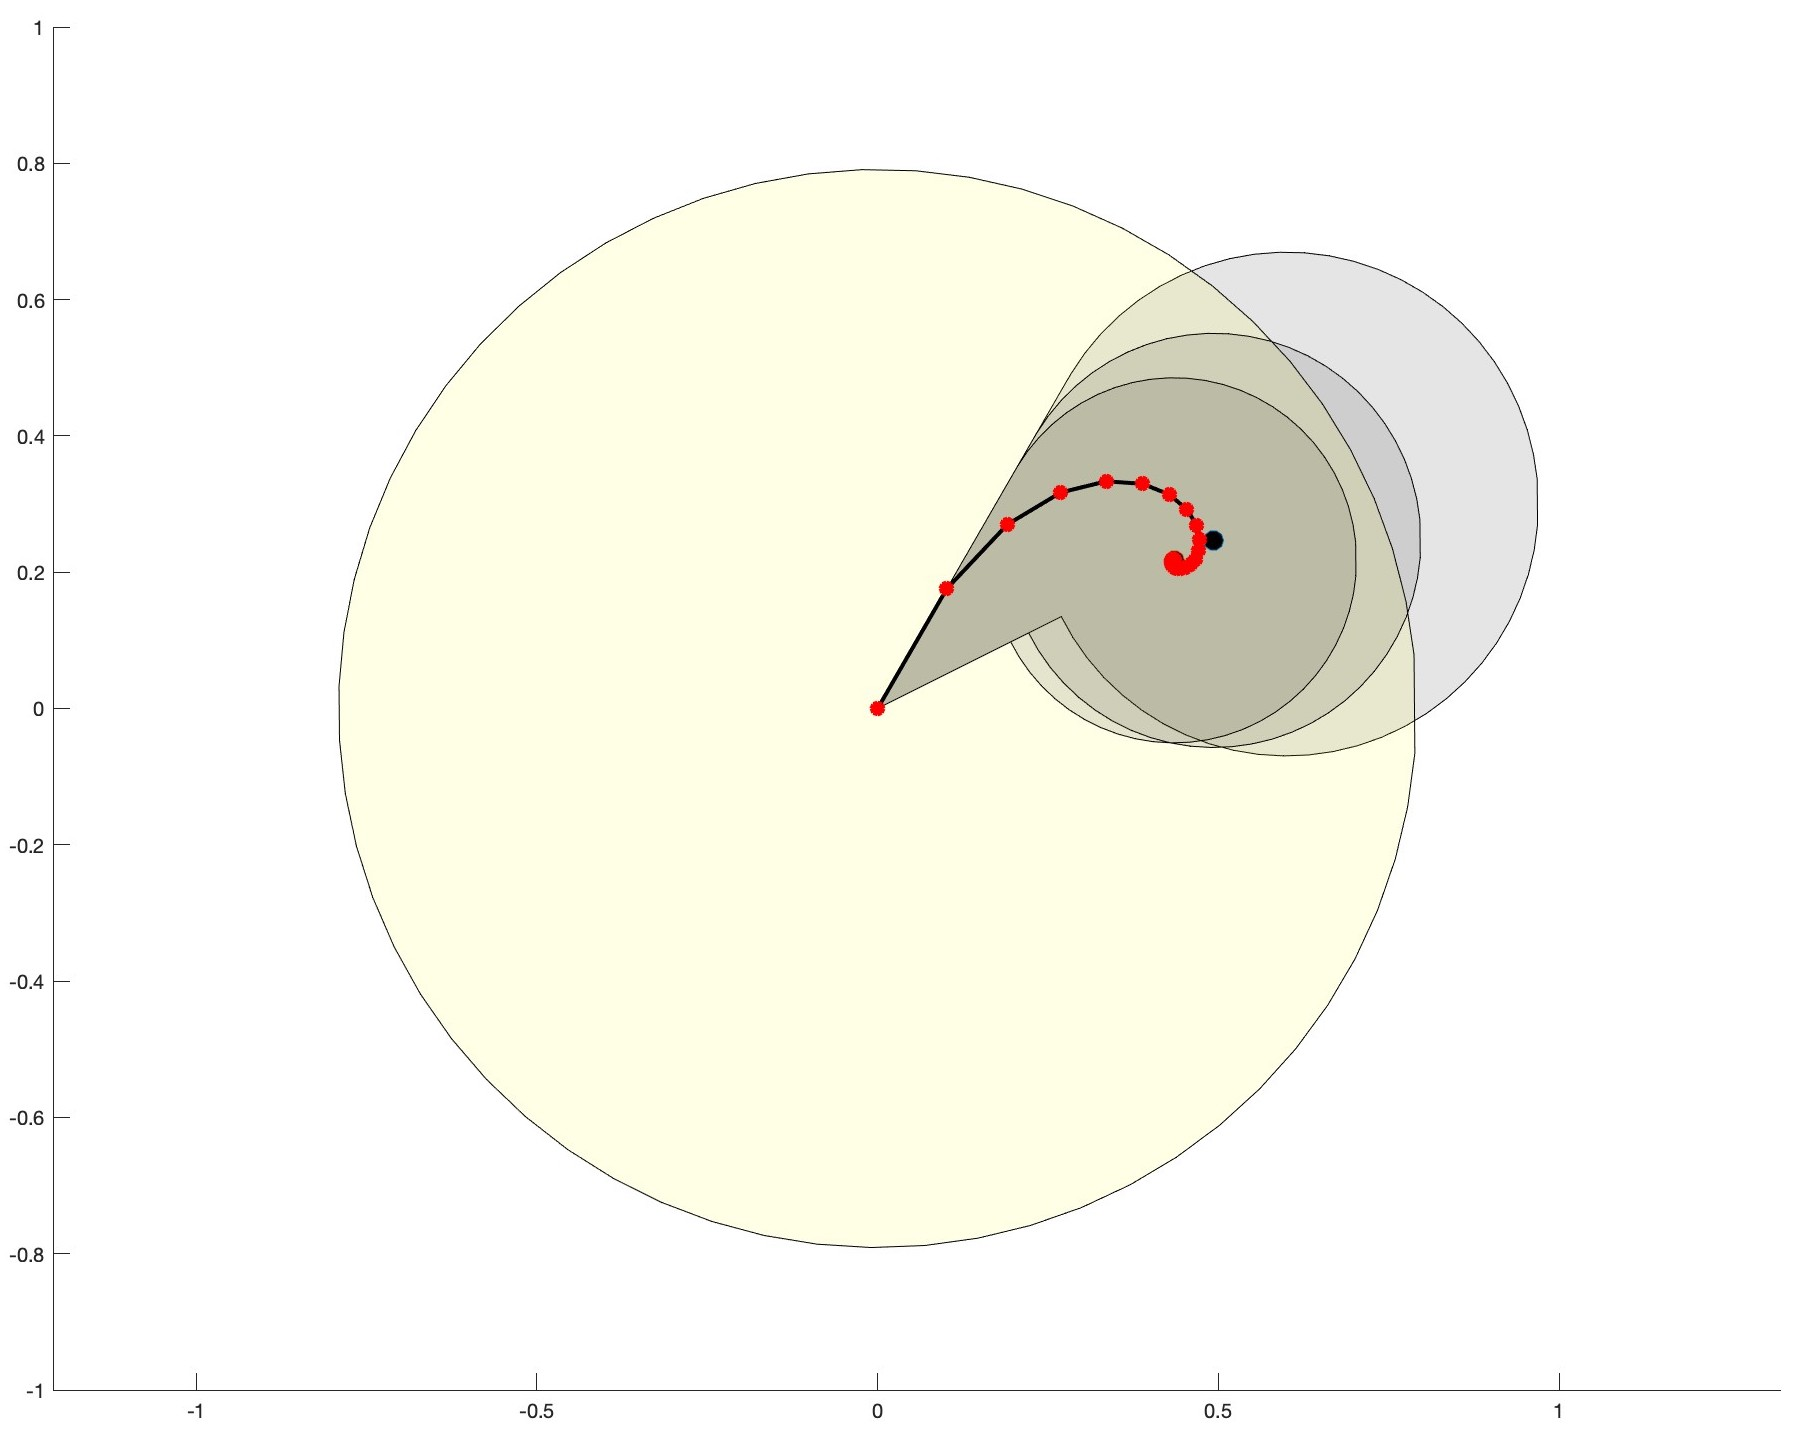
\includegraphics[scale=.07]{images/mot_pred.jpg}}
    \caption{Feedback Motion Prediction area for non-linear dynamics.}
    \label{fig:motion_pred}
\end{figure}

As already mentioned in the section \ref{unicyle}, the forward velocity is saturated to be at minimum zero, so that the parachute can never move backward but it is not forced to move at a minimum velocity in any case as happen in the real chutes. This assumption simplifies the control, becasue in the case of non-zero positive minimum velocity, \textcolor{blue}{and at least with this controlp policy} there is no guarantee that the parachute will not exit the Voronoi cell, for example when it is too close to the boundary.\\
\textcolor{blue}{To make sure that the parachute will not violate the Voronoi cell boundary, the FMP is initially calculated and, if it exits the cell, the arrival point (i.e. the new centroid founded by (\ref{centroid})), is moved closer to the actual position of parachute iteratively until the FMP fits into the Voronoi cell (as could be seen in \autoref{fig:motion_pred}).\\
\cite{b4} proposed differnt wais to define valid FMP areas, and among them it is chosen the \textit{Truncated Ice-Cream Motion Cone}, because it is the less conservative but smaller.}
\section{Implementation details}\label{sec:implementation_details}

\textcolor{blue}{\subsection{Structure of the simulations}
The simulations can be considered as composed by four different parts.
\subsubsection{Initialization}
The parachutes are initially randomly located around a desired point. They have to be properly spaced since the collision avoidance during the navigation is ensured only if they don't collide in the initial step,a nd because it is expected that real parachutes are delivered reasonably far from each others. \\
At the beginning of the simulation each parachute is aware of the number of agents in the swarm, it knows its own position with a small uncertainty, it does not know the position of all the other agents (and so it assigns a high uncertainty to them).
\subsubsection{Free falling}
The parachute after the launch begin to accelerate until their terminal velocity. In this section, the parachutes are closed and the input is set to zero. Only the wind disturbance can act on their position.
\subsubsection{Target convergence and controlled movement}
When the terminal velocity is reached the parachutes open and they begin to communicate each other, do the Voronoi tessellation and compute the input.
\subsubsection{Landing}
When the agents arrive at 1/10 of the initial height, they start to decelerate by breaking to reach the minimum vertical velocity, not to arrive at the ground too fast.}

\subsection{Localization}
Following the hypothesis mentioned in the \autoref{subsec:solution_localization}, the measurement error, GPS tracking and wind noises/errors have been set with zero mean and Gaussian, using a random variance generator. The values of the standard deviations have already been discussed in the section \ref{communication}.\\
While the dynamics take into account the wind effect, in the predictions step of the Kalman Filter it is supposed to be unknown; the parachute cannot in fact measure the direction of the wind and its module. However, the variance of the wind disturbance is supposed to be known, and it is included in the update of the covariance matrix of the estimated position (\ref{covariance}). In the equation are involved the model matrices $A$, $B$ and $G$ and the covariance matrix of the wind disturbance $L$, while the wind effect is set to zero.
\begin{gather}
    \label{prediction}
    x_{est} = Ax_{est}+Bu+G\begin{bmatrix}
        0 & 0 & 0 & \bar{v}_z
    \end{bmatrix}^T\\
    \label{covariance}
    P_{est} = AP_{est}A^T+BQB^T+GLG^T
\end{gather}
The same holds for the non-linear model, with the difference of having an EKF with linearized model matrices.\\
On top on what was already presented in \autoref{subsec:solution_localization}, another feature that have to be taken into account is the possibility for the agent \textit{i} to see \textit{j} at one time step but not in the following. When this happens, \textit{i} assumes that \textit{j} is still using the input of the last communication and so uses it to propagate the dynamic, while it increases the uncertainty. This update goes on up until when \textit{j} is seen again or the uncertainty on \textit{j} grows above a pre-defined threshold. Note that this propagation requires that during the data communication also the applied inputs are exchanged.

\subsection{Local estimation of the global centroid}
Each agent performs a local estimation of the global centroid by a weighted mean of the localization of the others by the uncertainty on them. This implies that if a parachute does not know the position of any other (which is equivalent that it knows the positions with high uncertainty), then it assumes that the centroid of the storm is itself and so it applies the hijh level control law only on itself. 

\subsection{Collision avoidance}
Without losing generality, let us assume that the agent \textit{i} is the one performing the tessellation, while \textit{j} is a different agent in the storm. Chute \textit{i} has location $p_i=\left[x_i, y_i, z_i\right]^T$, a physical dimension inscribed in a circle of radius $\delta_i$ in the horizontal plane and $\delta_{z,i}$ in the vertical one, knows its own position and the one of j with an uncertainty of respectively
{\small
\begin{equation*}
  diag(P_i^i)=\{{ \sigma_{x,i}^{i}}^{2}, {\sigma_{y,i}^i}^{2}, {\sigma_{z,i}^i}^{2}\}, \,  diag(P_j^i)=\{{\sigma_{x,j}^i}^{2}, {\sigma_{y,j}^i}^{2}, {\sigma_{z,j}^i}^{2}\}
\end{equation*}
}

where $P_i^i$ and $P_j^i$ are the covariance matrices of the localization error of \textit{i} and \textit{j} respectively, 
and has a maximum linear velocity of $v_{max,i} \ \left[\si{\meter\per\second}\right]$ in the horizontal plane and $v_{max,zi} \ \left[\si{\meter\per\second}\right]$ in the vertical (such that the maximum displacement in one time step is $s_i=v_{MAX,i}dt \ \left[\si{\meter}\right]$ and $s_{z,i}=v_{MAX,zi}dt \ \left[\si{\meter}\right]$ respectively) . 

\subsubsection{Uncertainty in the localization} 
  The uncertainty in the self localization is taken into account by increasing the dimension of the agent $\delta_i$ as:
    \begin{equation}
        \tilde{\delta_i}=\delta_i + \kappa \max \left\{\sigma_{x,i}^i, \sigma_{y,i}^i \right\}
        \label{eq:expand_dimension}
    \end{equation}
    where $\kappa$ is a coverage factor.\\
    The uncertainty on the position of \textit{j} is considered by projecting its location as:
    \begin{equation}
        \tilde{p_j} = p_j + \min\left\{ \lVert p_i-p_j \lVert, \kappa \max\left\{\sigma_{x,j}^i, \sigma_{y,j}^i\right\}\right\}\frac{p_i - p_j}{\left\lVert p_i - p_j \right\lVert}
    \end{equation}
   The use of the min function is necessary to avoid that the new agent \textit{j} position goes behind the agent \textit{i} itself.   
    
    \subsubsection{Finite dimension and discrete time dynamic}
    The finite dimension is taken into the picture by redefining the voronoi area as follows:
    \begin{gather}
        \tilde{\mathcal{V}_i} =
        \begin{cases} 
            \left\{ q \in \mathcal{Q} \lvert \left\lVert q-p_i \right\rVert \leq \left\lVert q-\tilde{p_j} \right\rVert\right\}  & \Delta_i \leq \frac{\left\lVert p_i - \tilde{p_j} \right\lVert}{2} \\
            \left\{ q \in \mathcal{Q} \lvert \left\lVert q-p_i \right\rVert \leq \left\lVert q-\hat{p_j} \right\rVert\right\} & \text{otherwise} 
        \end{cases} 
        \label{eq:voronoi_finite_dimensions}
    \end{gather}
    where $\Delta_i = s_i + \delta_{i}$ and
    \begin{equation}
        \hat{p_j} = \tilde{p_j} + \text{min}\{2 \delta_i, \left\lVert p_i - \tilde{p_j} \right\lVert\}\frac{p_i - \tilde{p_j}}{\left\lVert p_i - \tilde{p_j} \right\lVert}
    \end{equation}
    Moreover in the case when the centroid can reach the cell limit in one time step, the sensing range $R_s$ has to be reduced implying that the maximum voronoi cell is shrinked at least of the dimension of the chute:
    \begin{equation}
        \tilde{R_s} = 
        \begin{cases}
            R_s & \text{if } s_i + \delta_i > R_s\\
            R_s - \tilde{\delta_i} & \text{otherewise}
        \end{cases}
        \label{eq:rs}
    \end{equation}\\
    Note that this approach requires only the knowledge of the dimension of the chute performing the tessellation.

   \subsubsection{Decentralization of the algorithm} 
    In the decentralized implementation of the algorithm, it is possible that the chute is not aware of the location of all the others in the storm and so it has to care only about the parachutes that are in a region of space around it. This subset of agents is called \textit{neighbour set} and it is defined as:
    \begin{equation}
            \mathcal{N}_i = \left\{\hat{p_j} \in \mathbb{R}^2 \lvert \left\lVert p_i-\hat{p_j} \right\rVert < \tilde{R_{c,ij}} \right\}
            \label{eq:neighbour_set}
        \end{equation}
    with $\tilde{R_{c,ij}} = R_c + \kappa \left(\text{max}\left\{\sigma_{x,i}^i, \sigma_{y,i}^i\right\} + \text{max}\left\{\sigma_{x,j}^i, \sigma_{y,j}^i\right\}\right)$ in order to take into account also the uncertainties in the localization. With this consideration in mind, the agent's cell is given by:
        \begin{equation}
            \hat{\mathcal{V}_i}=\left\{\tilde{\mathcal{V}_i} \cap \bar{\mathcal{C}}_{i, \tilde{R_s}} \right\}
        \end{equation}
    where $\bar{\mathcal{C}}_{i, \tilde{R_s}}$ is the closure of the circle with radius $\tilde{R_s}$.  
    
    \subsubsection{Extension to the 3D case}  
    It is assumed that the agent performing the tessellation is able to detect the presence of the others even when they are above and below it in a range defined by $R_{cv}$ (sensing range in the vertical direction). In particular, when another agent is detected within this range it is included in the neighbour set as:
    \begin{gather}
        \tilde{\mathcal{N}_i} = \{p_j \in \mathcal{N_i} \lvert \lvert \Delta_z \lvert < R_{cv} + \kappa \sigma_z^i
        + \frac{\Delta_z}{\lVert \Delta_z \lVert }\Delta s_z\} %\notag
        \label{eq:neighbour_set_voronoi}
    \end{gather}
    where $\Delta_z=z_i - z_j$ is the height difference, $\Delta s_z = s_{z, i} - s_{z,j}$ is the difference between the maximum vertical displacements, and $\sigma_z^i=\sigma_{z,i}^i + \sigma_{z, j}^i$.\\
    Since the parachute models have only a unidirectional actuation in the vertical direction (i.e. they can only brake their fall and not go upwards) then the only limit that is necessary to identify for the z-axis tessellation is the lower. This can be done by:
    \begin{equation}
    {\scriptsize
        \mathcal{Z}_i = 
        \begin{cases}
            \left\{q\in \mathcal{Q} \lvert 0 \le z_i-z_q \le \Delta z - \delta_z - \kappa \sigma_z^i \right\}& \Delta_z \ge 0 \wedge i \in \tilde{\mathcal{N}_i} \\
            \left\{q \in \mathcal{Q} \lvert 0 \le z_i-z_q
            \le R_{sv} + \kappa \sigma_{z, i}^i \right\} & otherwise
        \end{cases}   } 
    \end{equation}
    where $z_q$ is the generic point along the z-axis.
   
\subsection{High-level motion control}\label{sec:details_high_level}
\subsubsection{Weights for the LQR}
The only parameters to be set in the LQR control are the weight matrices $S$ and $R$. By increasing the state matrix the algorithm tries to reduce the error between the actual state and the desired one, while by increasing the input matrix the input is minimized. They are usually competing objectives. Since the parachute inputs will be saturated in the low level control, there is no interest in using a big input matrix, while is important to have a good performance of the states to reduce the final distance between the global centroid and the target.
\subsubsection{Same control for all the chutes}
As said before this is the simples control low because the agents applys on itself the same input computed for the fake parachute representing the global centroid.
\subsubsection{Inverse kinematics}
 Regarding the inverse kinematics, in the postural task it is asks to make the single agents converge towards the global centroid, in order to reduce the root mean square of the agents distance from the global centroid end, eventually, from the target, thanks to the main task. The importance of this choice is explain further in the Results section.  When using the postural task, the weighting value is set such that the more the global centroid is close to the target, the more importance is given to letting the single parachute converge toward the global centroid, with an exponential behaviour. The pseudo-code of the inverse kinematics algorithm is presented in the Algorithm \ref{algorithm}.\\
\textcolor{red}{Decommentare l'algoritmo}
% \begin{algorithm}[hb]
% \caption{Numerical IK}\label{NIK}
%     \begin{itemize}
%     \item Find centroid error position $e_c$
%     \item Find parachute error position $e_x$
%     \item Find total error position $e=[e_c;e_x]$
%     \item Find jacobian matrix $J$
%     \item Initialize line search factor $\alpha=1$
%     \item Initialize weighting factor $w$
%     \end{itemize}
%     \mywhile \ $|e_c|^2 \ge 0.5 \And |e_x|^2 \ge 0.1$
%     \begin{enumerate}
%         \item $\Delta x = (J^TJ+w^2I)^{-1}(J^Te_c+w^2e_x)$
%         \item $x_{test} = x + \alpha \Delta x$
%         \item $x = x_{test}$
%         \item $e = e'$
%     \end{enumerate}
%     \myendwhile
%     \label{algorithm}
% \end{algorithm}

\subsubsection{Managing of emergency case}
\textcolor{blue}{
As said before, the low level control is performed after having divided the plane where the parachute moves with a voronoi tessellation considering all the agents that are in a sorrounding space of the considered one. Even though it is in principle admissible for two agents having the same psition in the xy plane and different heigh, there are some situations in which this can create problems. For example, when an agent sees many others around it, its voronoi cell may be reduced to a point because having considered uncertinities and finite dimensions. If in this case it localize other agents below it with a xy location reasonably close to its own, then it will be not able to move to avoid the collision. To solve this issue, the \textit{emergency control} tries to move the falling agent as far as possible from the new see ones. This is done by not considering the uncertinties in the tessellation (i.e. enlarging the voronoi cell as much as possible) and moving in the opposite directions with respect to sum of the vectors connecting itself and the considered ones.}
\subsection{Low-level motion control}
While the value of the LQR gain is calculated by the algorithm, the values of the proportional gains of the low-level control have to be chosen. For the linear model gain of the equation (\ref{eq:proportional}) it is important to choose a value such that there is no risk of overshooting the target. This condition is avoided if the inequality (\ref{gain}) holds: in one step the displacement given by the controller must not be greater than the target distance.\\
\begin{equation}
  k_p\left(p_i - C_{\mathcal{V}_i}\right)dt \le \left(p_i - C_{\mathcal{V}_i}\right) \Rightarrow k_p \le 1/dt
  \label{gain}
\end{equation}
For what concerns the non-linear model, on the other hand, the gain for the forward velocity is set to one and the gain for the angular velocity is set such that in one time step it is less than the maximum one (\ref{angular_vel}).
\begin{equation}
  \label{angular_vel}
  k_{\omega} = \omega_{max}/\pi
\end{equation}
\textcolor{blue}{Once the input are calculated and error is sum to them in order to take into account their errors, and the they are saturated to consider the real performances. Even tough the real actuator has not been identified the errors' standard deviation of the actuators are set as 10\% of the maximum admissible input, with a coverage factor of 3 (i.e. 99.73\% of probability).}

\subsection{Conclusion of the simulation}
When an agent touches the ground it cannot move any more, and its control input is set to zero. However, the GPS signal continues to arrive and the parachute continues to communicate with the other agents and to send its own position.
\section{Results}
\subsection{Test of the Voronoi tessellation}
Even though the Voronoi tessellation is performed in the 3D space, an example of implementation for two agents in the 2D plane is here presented in \autoref{fig:Voronoi_example} because it is more understandable. The communication ranges are $R_{c1}=2.2, R_{c2}=0.55$ and a coverage factor of $\kappa=3$ has been used.  Here three different cases are reported: A) agents with point dimensions and $s_{max}=0$ (i.e. analogous to the continuous time implementation of the algorithm) and perfect localizations, B) finite physical encumbrance $\delta_1=0.25$, $\delta_2=0.15$, finite space $s_{max,1}=1$, $s_{max,2}=0.35$ and perfect localization, C) finite physical encumbrance, finite velocity and uncertainty in localization $\sigma_{1}^1=\sigma_{2}^2=0.05^2 \text{\textit{I}}_3, \sigma_{1}^2=0.1^2 \text{\textit{I}}_3, \sigma_{2}^1=0 \text{\textit{I}}_3$.
\begin{figure}[htb]
\centering
    \includegraphics[width=0.7\columnwidth]{images/fig_Voronoi_example.eps}
    \caption{Example of the Voronoi tessellation for two agents in the plane. $\mathcal{V}_A$ is build considering only the position of the agents, $\mathcal{V}_B$ considers finite dimensions and velocities while $\mathcal{V}_C$ considers also the uncertainties.}
    \label{fig:Voronoi_example}
\end{figure}
In case A, agent \textit{1} sees \textit{2} inside its communication range and sets its cell limit at half their distance; chute \textit{2} does not see \textit{1} and so its cell becomes the whole circle with radius $R_{c2}$. In case B, agents \textit{1} and \textit{2} in one-time step can reach the limit of the cell, so they have to shrink their old cells of $\delta_1$ and $\delta_2$. The Voronoi limit of agent \textit{2} moves inside the encumbrance of the chute itself. In case C, on top of what already happened in case B, \textit{1} further shrinks its limits so that in the direction between \textit{1} and \textit{2} the limit goes above \textit{1}. Meanwhile, \textit{2} increases its encumbrance, reducing its Voronoi limit more than the dimension of the previous area, leading the final cell to be a point. In that final condition, \textit{1} cannot move towards while \textit{2}, while \textit{2} cannot move at all.

\subsection{Example of localization}\label{subsec:ex_localization}
\autoref{fig:fig_self_update} reports an example of the localization done by one agent on itself when the EKF uses the GPS measurement and the model (labelled \textit{measure}) or only the latter (labelled \textit{model}). In this specific example, nine agents fall from $[500, 500, 1000]$ toward $[0,0,0]$, with the inverse kinematic enabled and the probability of having the GPS measure equal to 50\%. The iterations when the initial free-falling period and the landing on the ground are highlighted with dashed lines.
\begin{figure}[h]
\centering
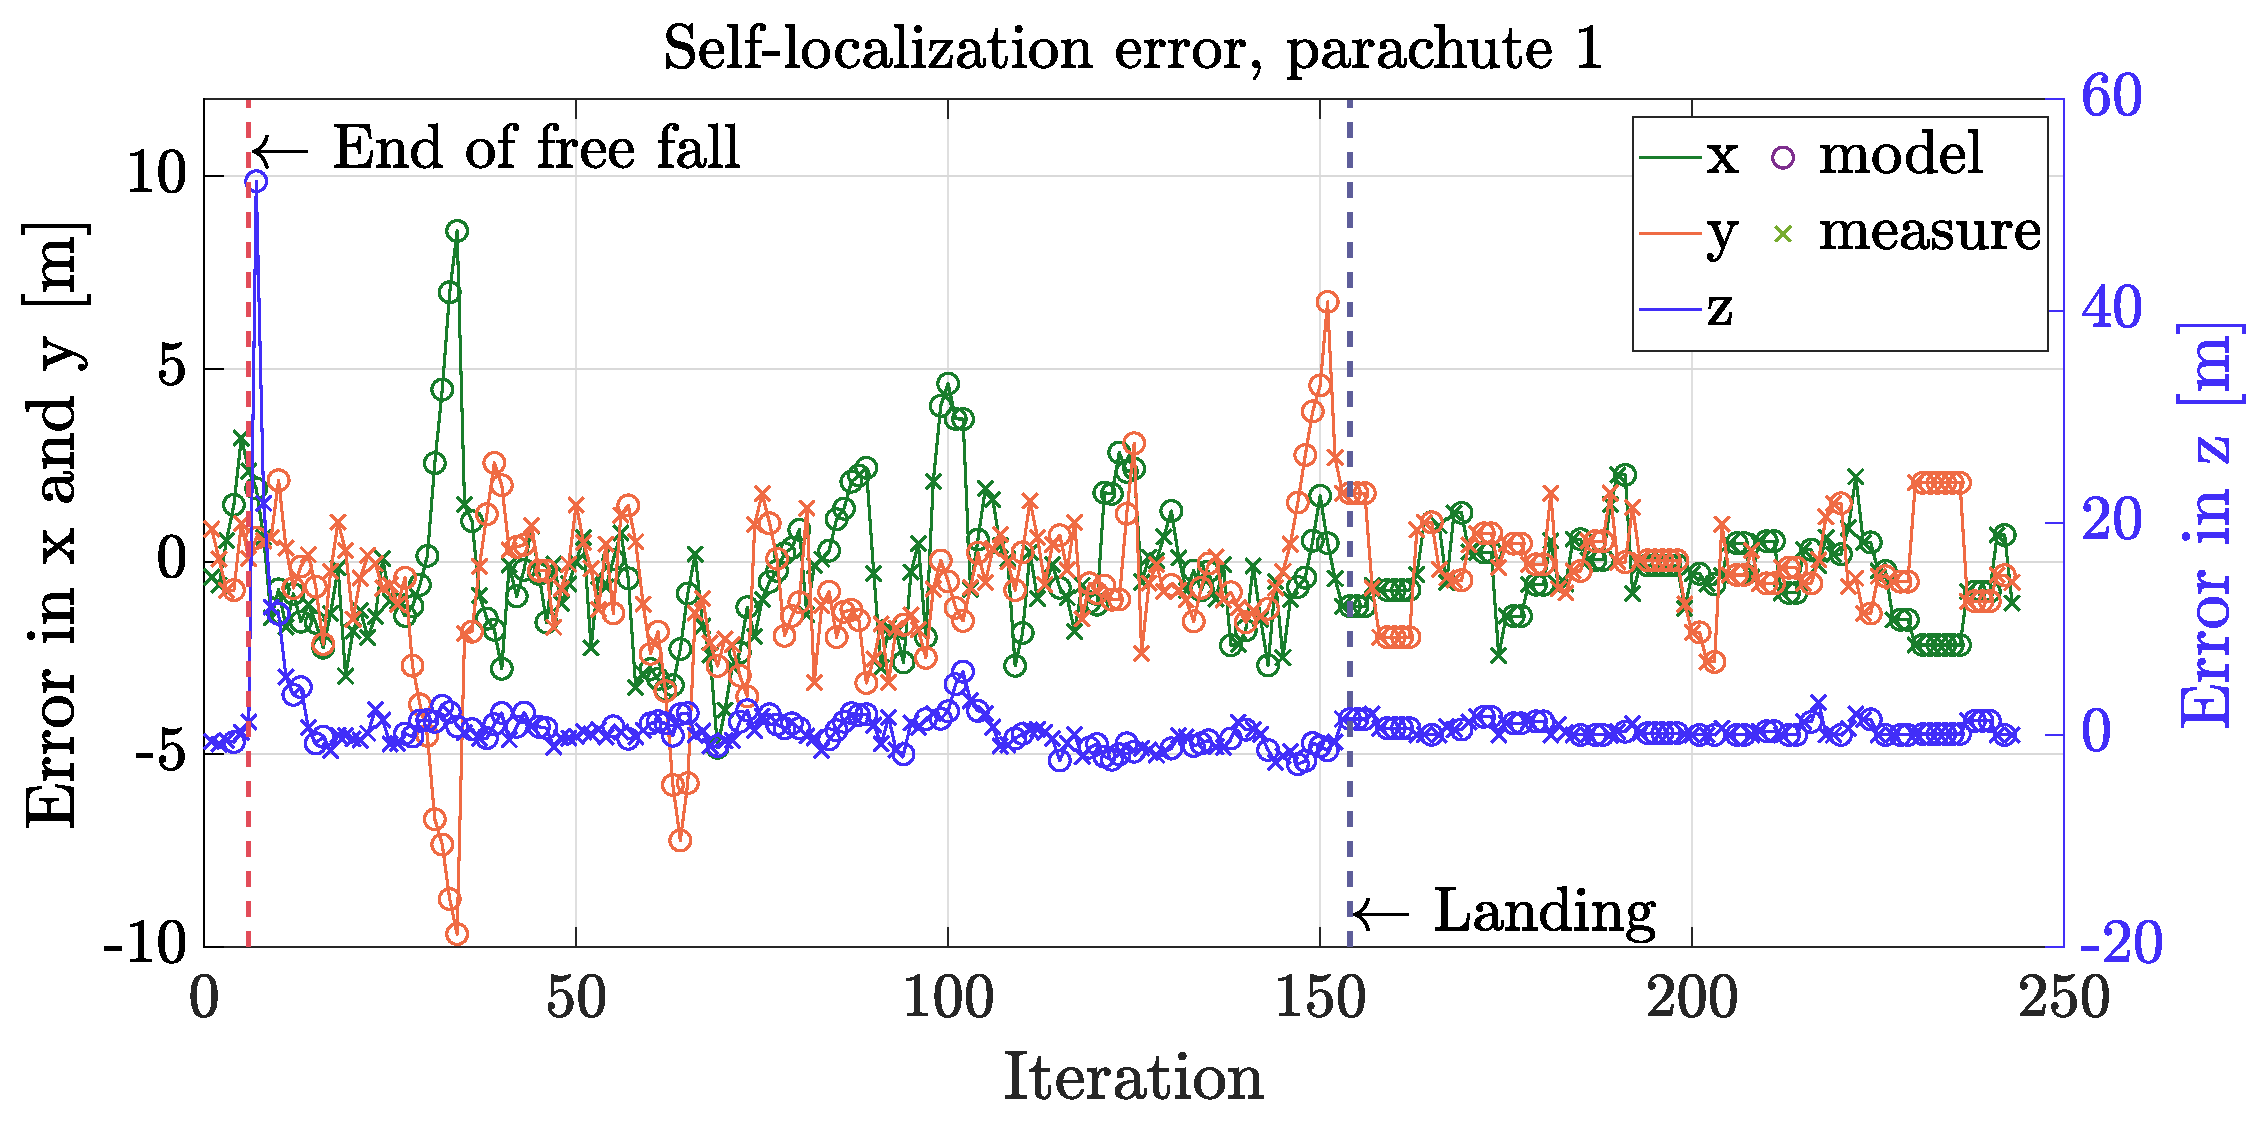
\includegraphics[width=\columnwidth]{images/fig_self_update.eps}
\caption{Error in the self-localization done by agent 1, with a probability of having the GPS measure of 50\%.}
\label{fig:fig_self_update}
\end{figure}
It could be seen that after the end of the free-falling part when the parachute opens and the falling velocity suddenly reduces, the localization error grows a lot, while it quickly decreases in a few iterations. It is also interesting to notice how there are no GPS measurements between iterations 27 and 34, so the error made by localizing with only the model grows. At iteration 35, a new GPS signal is available, and the error is reduced. Finally, the errors are lower after the landing because wind and input noises no longer affect the agent's position.
\subsection{Example of a complete swarm trajectory}\label{subsec:complete_sim}
\autoref{fig:3D_traj} shows the trajectory followed by 13 parachutes falling between the previous positions, while \autoref{fig:state} shows the time evolution of states and control inputs for one of the falling parachutes. The wind noise has been set to 3 $\left[\si{\meter\per\second}\right]$ in every direction.
\begin{figure}[h]
    \centering
    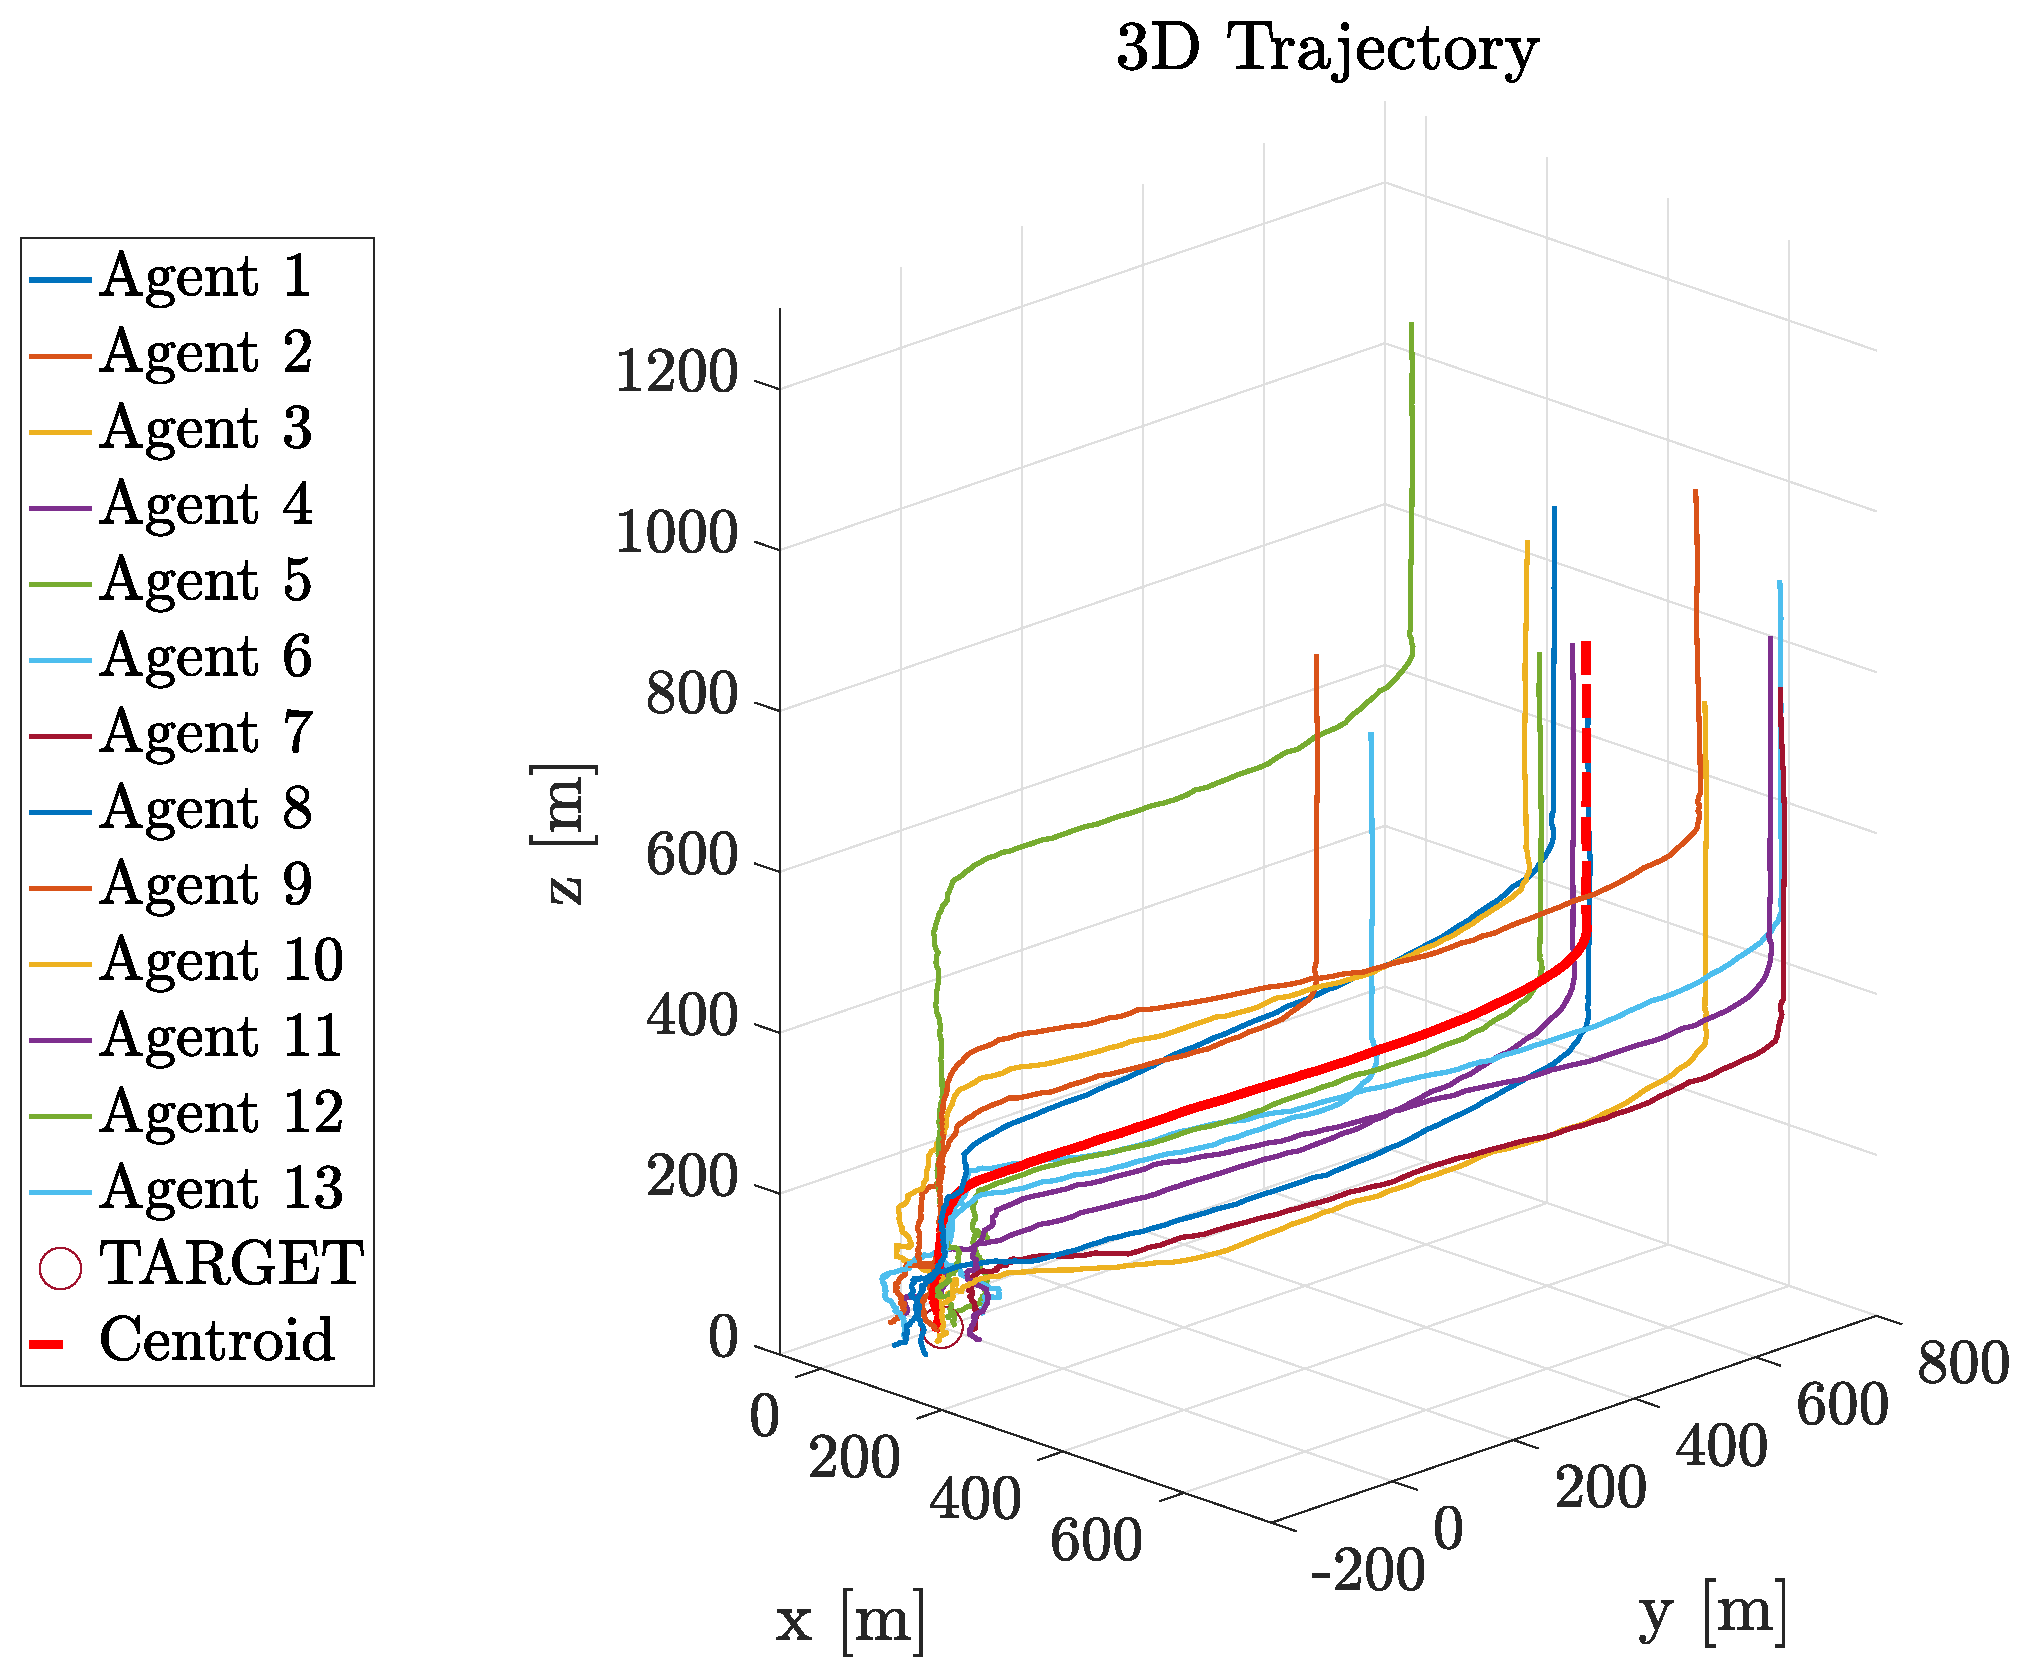
\includegraphics[width=\columnwidth]{images/fig_3D.eps}
    \caption{3D trajectory with 13 parachutes and all probabilities set to 1.}
    \label{fig:3D_traj}
\end{figure}
\begin{figure}[h]
    \centering
    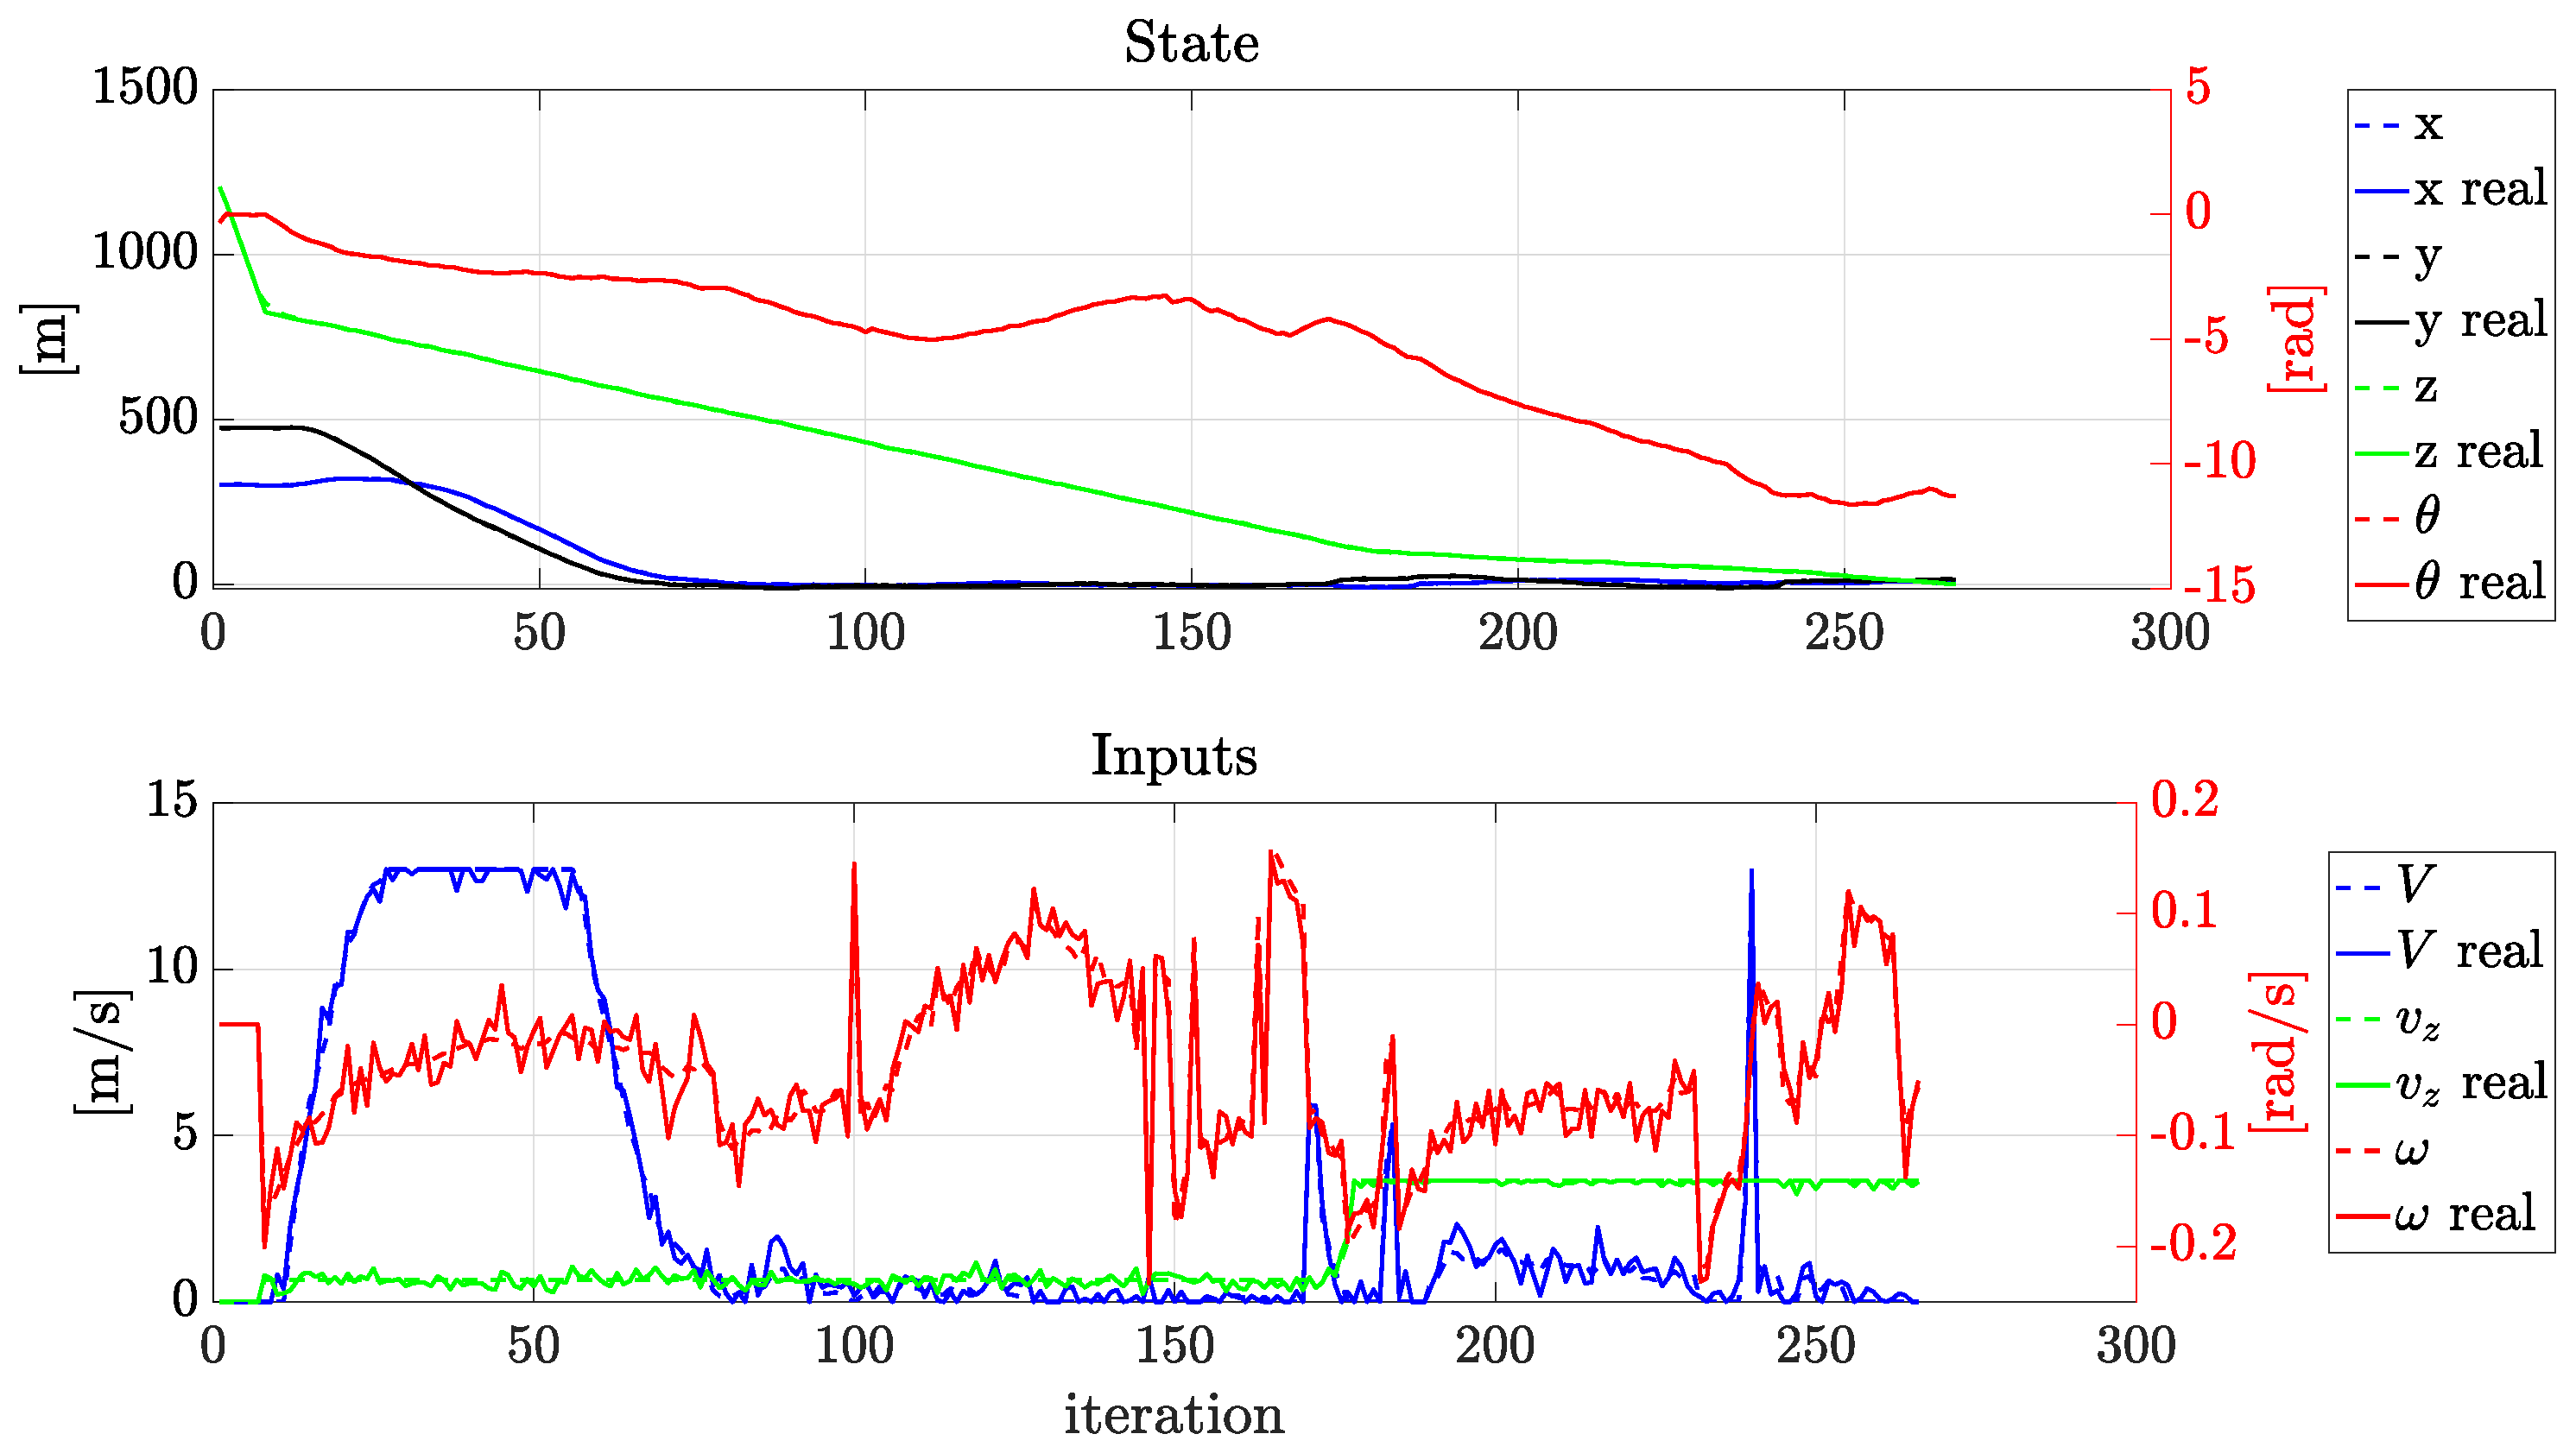
\includegraphics[width=\columnwidth]{images/fig_1.eps}
    \caption{States and inputs behaviour of agent 12.}
    \label{fig:state}
\end{figure}
It could be seen that the centroid (red dashed line of \autoref{fig:3D_traj}) reaches the target correctly, while the parachutes fall around it without any collision.\\
Regarding the inputs, it may be noticed that there is no actuation in the initial free-falling part. In contrast, in the final part, the control on the z-axis is saturated to reduce the speed before contact with the ground. Also, the forward velocity is saturated in the central part, where the agent moves toward the target. 

\subsection{Distributed WLS}
\autoref{fig:ab_IK} represents the standard deviation of the localization error committed by agent 7 of the simulation in \ref{subsec:ex_localization} in the localization of the others before and after distributing information via the WLS algorithm in the three directions. It must be noted that \textit{before WLS} considers the localization at the time steps when the relative distance measurement is performed or when the dynamic of the other is propagated through the model. On the other hand, \textit{after WLS} considers the result of the consensus algorithm, so in that instant, the localization can also be based only on the information shared by the network with the considered one.
\begin{figure}[h]
    \centering
    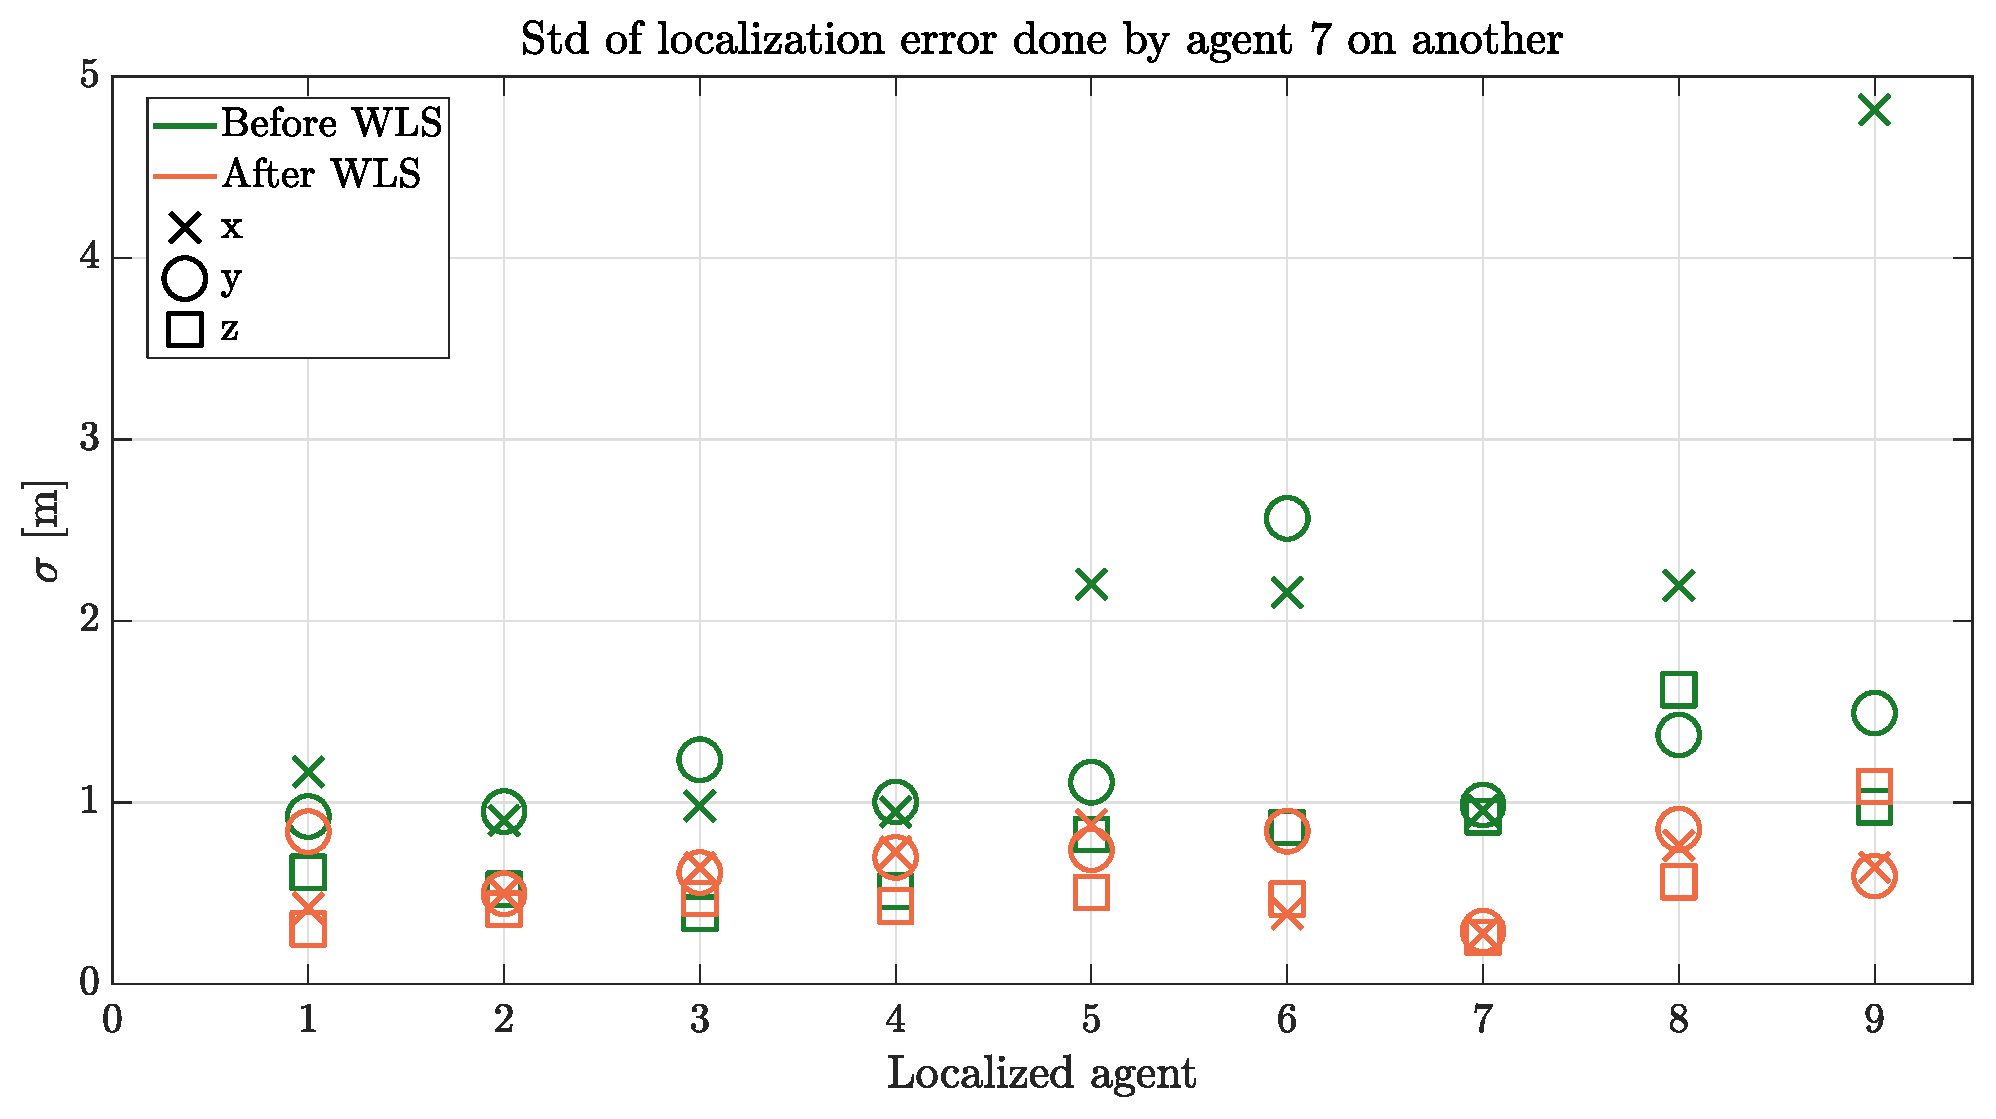
\includegraphics[width=\columnwidth]{images/mdl2_9chutes_be_wls.eps}
    \caption{Standard deviation of the error made by the parachute seven on the localization of the others.}
    \label{fig:ab_IK}
\end{figure}
Note that, as expected after the WLS, the error in the localization is reduced for all the agents.
\subsection{Effect of the Inverse Kinematics}
A comparative test has been done to test the IK's effectiveness in the navigation. In particular, several parachutes have been driven with and without using the IK. The initial conditions of the two cases are the same for a given round, and more rounds have been run. No uncertainties and noises have been introduced to highlight the effect of the navigation only. Finally, the distance between the centroid and the target has been computed alongside the agent's Root Mean Square (RMS) to the target distance. The mean results among multiple rounds are collected in \autoref{tab:IK_comparison}.
It could be seen that the IK approach reduces the dispersion of the chutes around the target, thanks to the postural task, for both models. In contrast, the distance of the global centroid from the target seems independent of the choice, except in the case of only one parachute. However, since having all the parachutes as near as possible to the target may be preferable, the RMS highlights the task's success.
\begin{table}[]
\scriptsize
  \caption{Comparison between the use of IK or not}
  \centering
  \begin{tabular}{ccccc|cccc}
  \hline
  & \multicolumn{4}{c}{Linear} & \multicolumn{4}{c}{Non-linear}\\
  \multicolumn{1}{c}{\#} & \multicolumn{2}{c}{Dist.} & \multicolumn{2}{c}{RMS} & \multicolumn{2}{c}{Dist.} & \multicolumn{2}{c}{RMS}\\
  \multicolumn{1}{l}{}  & IK & No IK & IK & No IK & IK & No IK & IK & No IK \\ \hline
  1   & 2.99 & 0.01 & 2.99 & 0.01 & 3.00 & 0.02 & 3.00 & 0.02  \\
  3   & 6.21 & 3.05 & 25.36 & 33.34 & 7.72 & 4.42 & 25.36 & 27.74 \\
  5   & 4.32 & 6.13 & 29.41 & 38.76 & 6.86 & 5.61 & 32.84 & 39.83 \\
  7   & 3.07 & 4.86 & 35.20 & 41.88 & 6.30 & 4.57 & 32.62 & 47.31 \\
  9   & 5.12 & 5.47 & 37.56 & 49.35 & 7.21 & 8.64 & 41.49 & 48.43 \\
  11  & 2.31 & 2.53 & 43.18 & 53.43 & 8.83 & 5.90 & 43.44 & 55.80 \\
  13  & 4.70 & 3.47 & 46.37 & 58.23 & 3.42 & 7.52 & 46.91 & 57.78 \\
  \hline
  \end{tabular}
  \label{tab:IK_comparison}
\end{table}



\subsection{Effect of the probabilities}
A parametric study has been conducted changing the probability of having the GPS or relative measurements between chutes, which simulates the ability of the real devices to acquire the data. This simulation considers nine parachutes of the nonlinear type affected by noise. The initial free-falling part and the final deceleration are turned off in the simulation because the localization takes some iterations to recover the error induced by the sudden change of vertical dynamics. In each test, one of the probabilities has been changed while the other has been kept constant at 100\%. After the simulation, the standard deviation of the localization error in the three directions has been computed for the self-localization in \autoref{fig:self_loc} and on the others in \autoref{fig:other_loc}. For the latter case, the mean of the error on all the others is reported.
\begin{figure}[h]
    \centering
    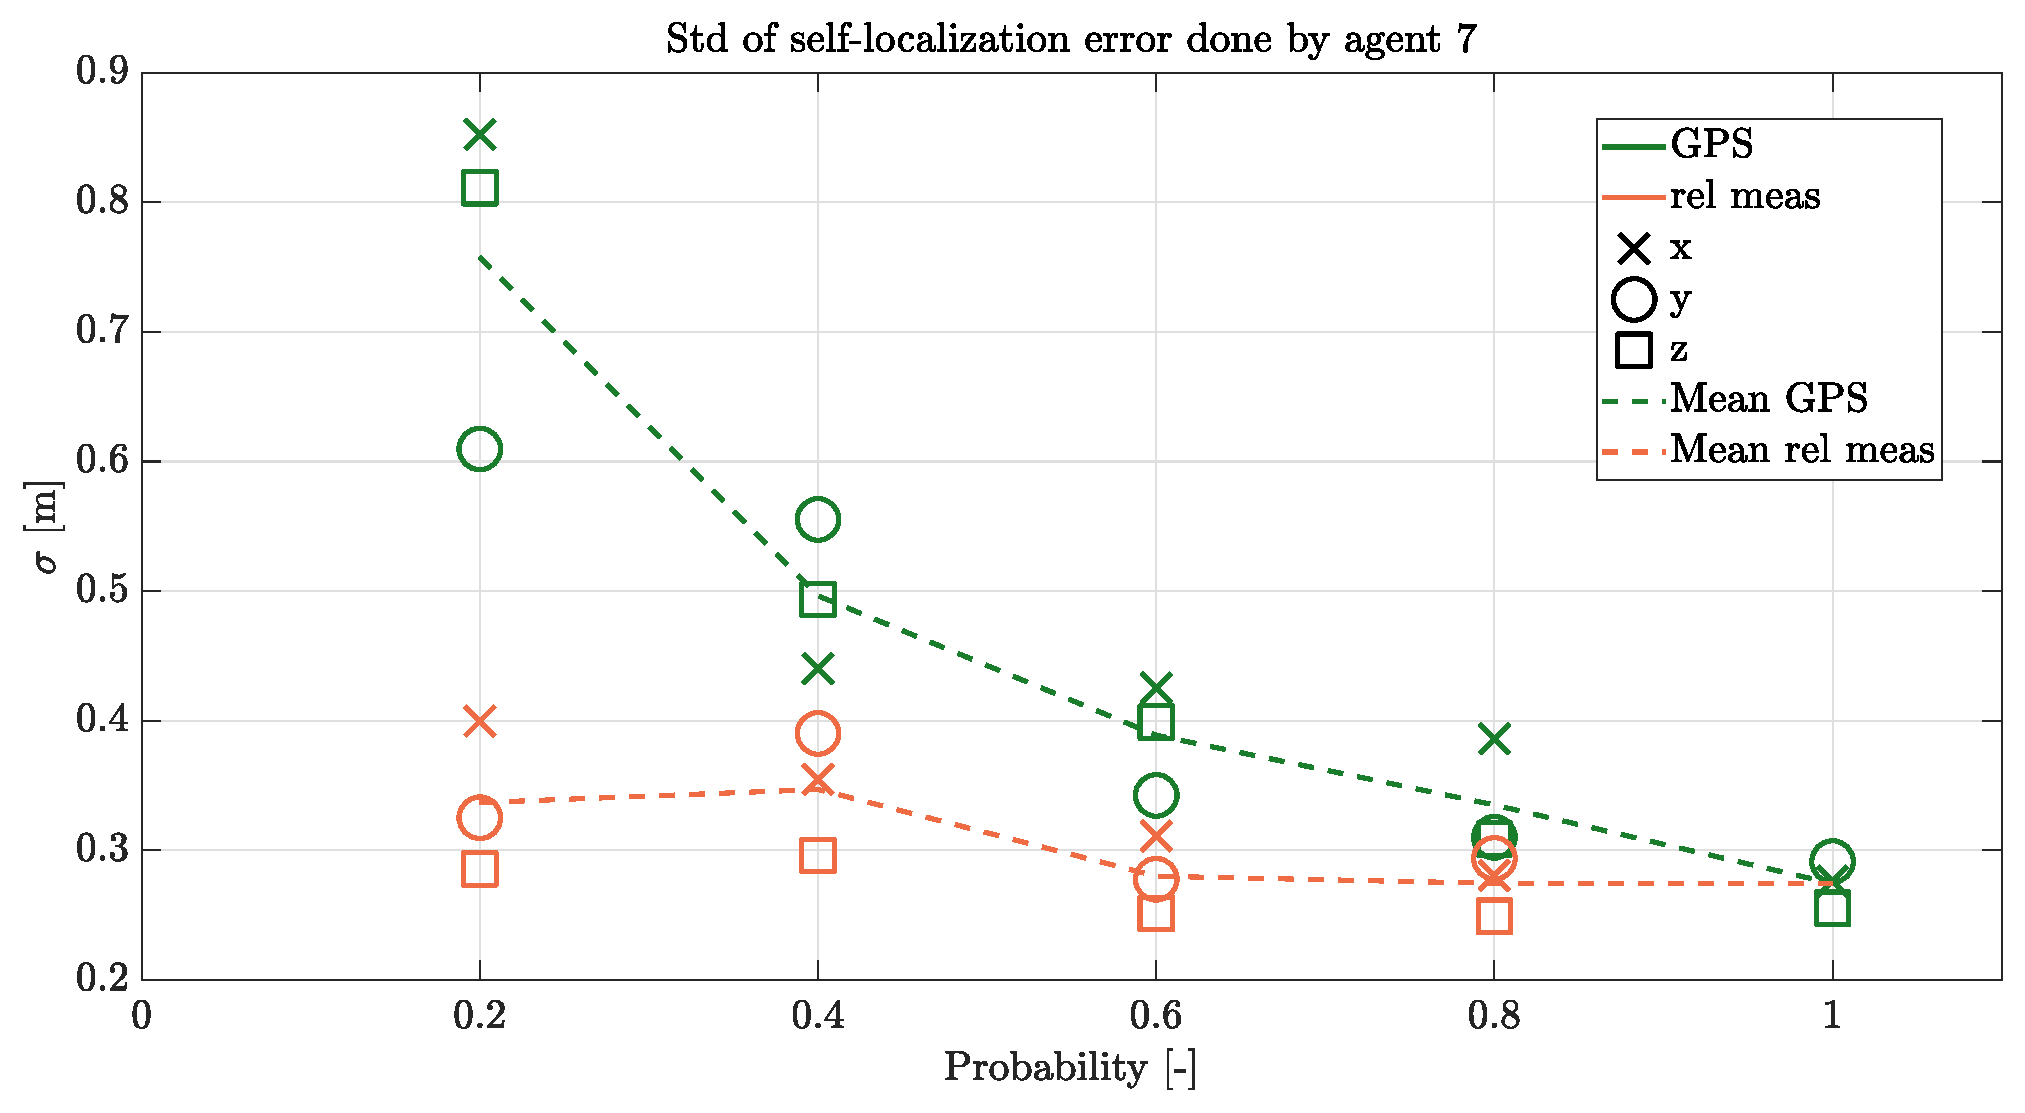
\includegraphics[width=\columnwidth]{images/mdl2_9chutes_parametric_beforeconsensus.eps}
    \caption{Standard deviation of the localization error made by the parachute seven on itself at different values of GPS and relative measurements probabilities.}
    \label{fig:self_loc}
\end{figure}
\begin{figure}[h]
    \centering
    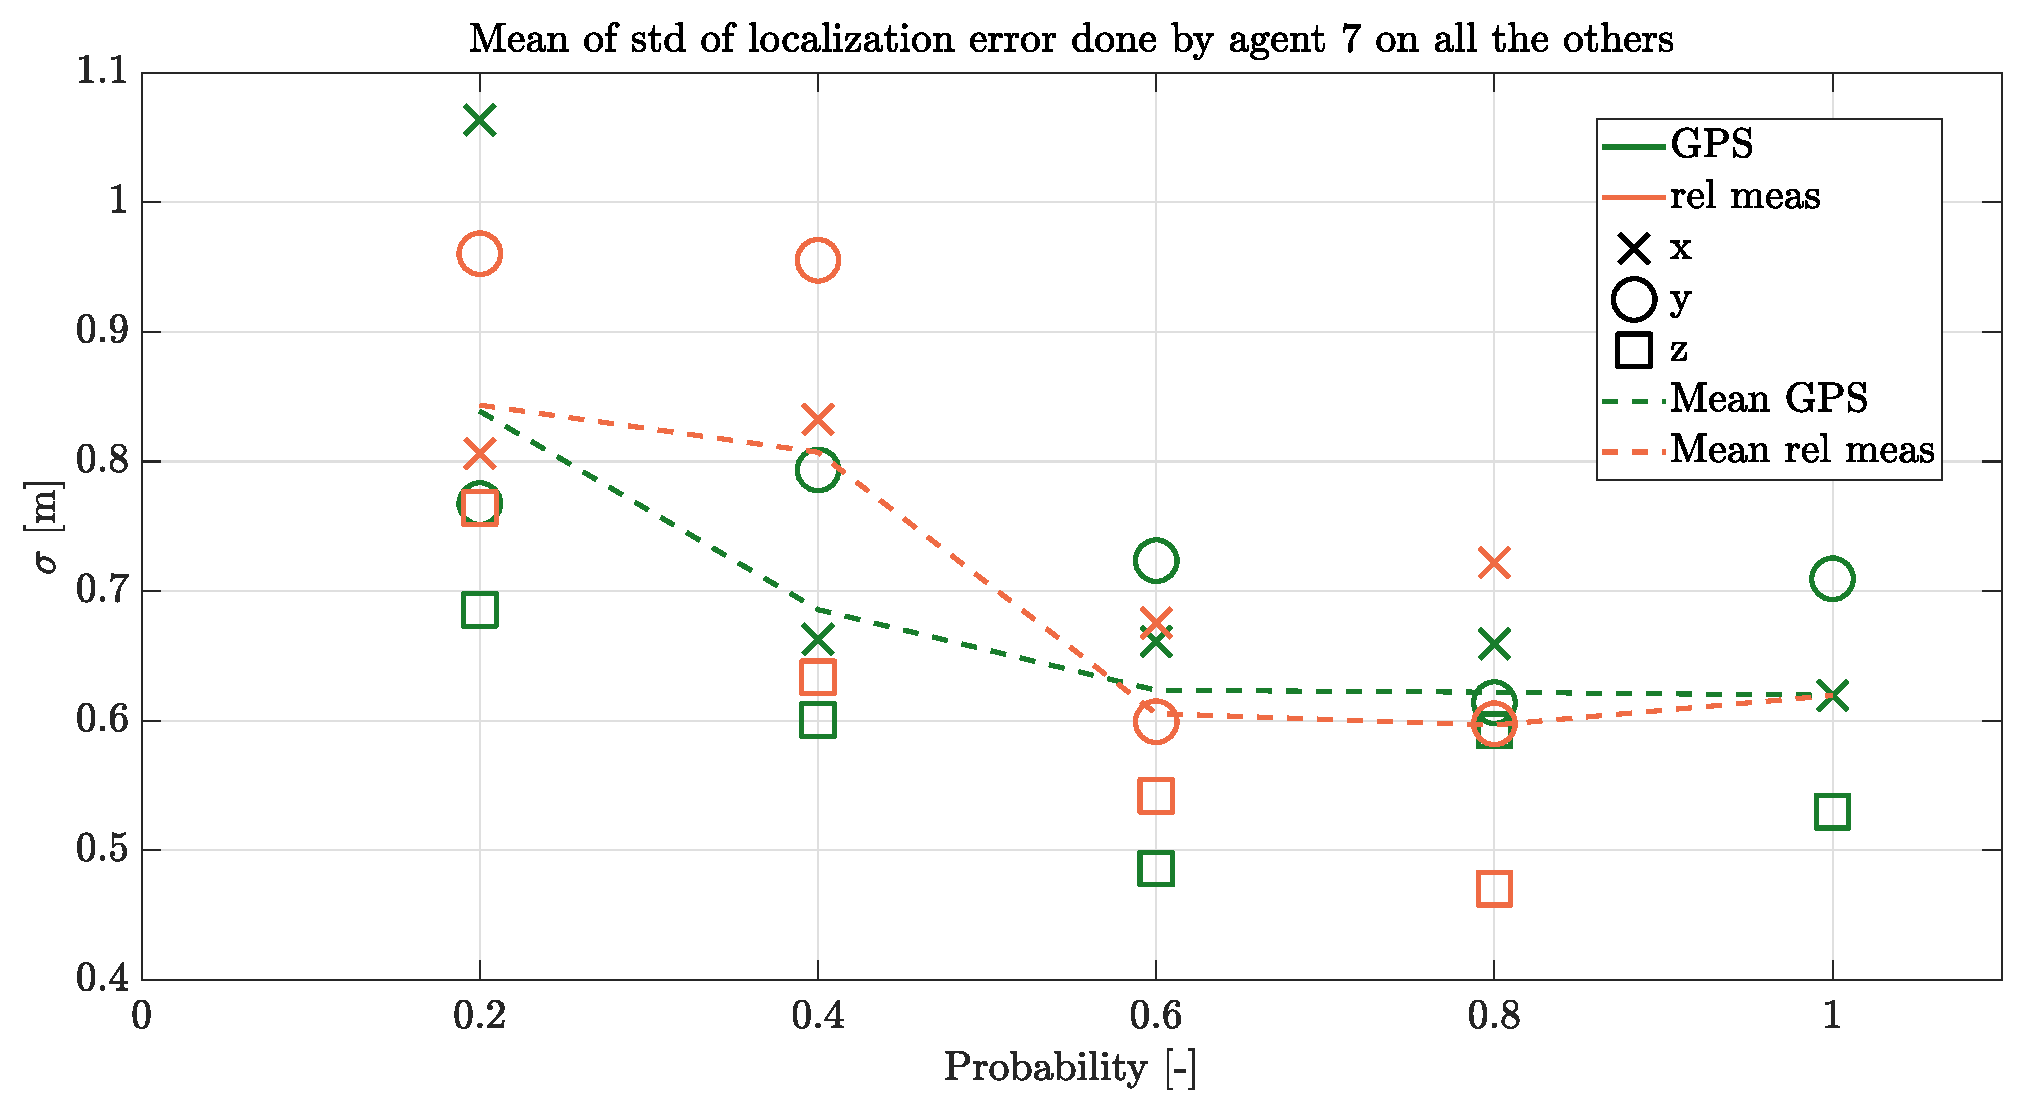
\includegraphics[width=\columnwidth]{images/mdl2_9chutes_parametric_loc_others.eps}
    \caption{Standard deviation of the localization error made by parachute seven on the other parachutes at different values of GPS and relative measurements probabilities.}
    \label{fig:other_loc}
\end{figure}
The graph shows that the GPS probability highly affects the self-localisation error, while it is less by the relative measurement. This may be due to two facts. The first is that the GPS alone can provide good localization, so the further information added by the relative measurement has a small contribution to the estimation. Furthermore, the probability of having the relative measurement is conditioned by the distance between agents, which in our simulation depends on its evolution.\\
On the other hand, the two effects are more combined in the localization errors made on the others since, for this analysis, the possibility of exchanging messages rules the process. In fact, when the agents are not close enough, they cannot exchange information with one another. Hence, the collected information (independently from its source) cannot be shared, and no contribution can be provided to the localization. Furthermore, when the connectivity is not always ensured, the effect of the error committed by propagating the states with the model is more significant.
\section{Conclusion}
The project objectives been fulfilled with success, since the centoid of the parachute storm has been correctly driven from the initial point to the ground target. The prescribed centroid trajectory has been computed with an optimal controller, while two wais to coordinate the agents' movement has been proposed. The employed parachutes were a simple linear model and a more complicated unicycle like nonlinear ones, so two different control laws has been studied for them. Finally, no collision between agents have been reported thanks to the employiment of a control law based on the voronoi tessellation. \\
Some aspects that can be included in the feature are:
\begin{itemize}
    \item The presence of a minimum forward speed at which tha parachute have always to fly;
    \item Consider the foces applied by real actuators instead of their overall effects on the velocities
    \item The possibility of unidirect communications, leading to non symmetric adjacency matrix; 
    \item Implementation of a fully 3D Voronoi cell able to manage all the cases of inclusion of agents in all the directions;
    \item Not discharging the self-localization information reached after the WLS round before using it in the new KF/EKF, this may be done ith some more advanced localization algorithm, such as the Cooperative localization as described in \cite{b14}.
\end{itemize}
\begin{thebibliography}{00}
\bibitem{b2} Martino, J., \& Setters, D. (2020, July 27). Precision Motors help guided parachutes deliver cargo. Tech Briefs. \url{https://www.techbriefs.com/component/content/article/tb/supplements/mct/features/applications/11837}

\bibitem{b3} Precision guided parachutes - maxongroup.us. Available at: \url{https://www.maxongroup.us/medias/sys_master/root/8803679404062/Precision-Guided-Parachutes.pdf?attachment=true} (Accessed: 01 July 2023).

\bibitem{b11} Ultra-Wideband RTLS, Positioning, \& Sensor Technology Available at: \url{https://www.inpixon.com/technology/standards/ultra-wideband#:~:text=What%20is%20the%20Range%20of,sight%20between%20devices%20or%20anchors.} (Accessed: 07 September 2023). 

\bibitem{b8} La velocità di un paracadutista con un paracadute aperto. Velocità di caduta del paracadutista. (no date) Kemtalant. Available at: \url{https://kem-talant.ru/it/bodybuilding/skorost-parashyutista-s-raskrytym-parashyutom-skorost.html} (Accessed: 21 August 2023). 

\bibitem{b9} La dimensione del paracadute. (no date) Kemtalant. Available at: \url{https://www.sportsrec.com/7305468/the-size-of-skydiving-parachutes} (Accessed: 21 August 2023). 

\bibitem{b7} Britannica, The Editors of Encyclopaedia. "parachute". Encyclopedia Britannica, 7 Aug. 2023, \url{https://www.britannica.com/technology/parachute}. Accessed 21 August 2023.

\bibitem{b10} F.A.Q. | Skydive Lucca (no date) Scuola di paracadutismo Lucca. Available at: \url{http://www.paracadutismolucca.it/f-a-q/} (Accessed: 21 August 2023). 

\bibitem{b12} Kim, Y., \& Bang, H. (2019). Introduction to Kalman Filter and Its Applications. IntechOpen. doi: 10.5772/intechopen.80600

\bibitem{b1} Manuel Boldrer, Luigi Palopoli, Daniele Fontanelli,
A unified Lloyd-based framework for multi-agent collective behaviours,
Robotics and Autonomous Systems,
Volume 156,
2022,
104207

\bibitem{b15} S. Ahmad and M. O. Tokhi, "Linear Quadratic Regulator (LQR) approach for lifting and stabilizing of two-wheeled wheelchair," 2011 4th International Conference on Mechatronics (ICOM), Kuala Lumpur, Malaysia, 2011, pp. 1-6, doi: 10.1109/ICOM.2011.5937119.

\bibitem{b5} Benhabib, B. \& Goldenberg, Andrew A. \& Fenton, R.. (2007). A Solution to the Inverse Kinematics of Redundant Manipulators. Journal of Robotic Systems. 2. 373 - 385. 10.1002/rob.4620020404. 

\bibitem{b6} Aristidou, A. \& Lasenby, J. Inverse kinematics: a review of existing techniques and introduction of a new fast iterative solver. (University of Cambridge, Department of Engineering,2009)

\bibitem{b4} İşleyen, A., Wouw, N. \& Arslan, Ö. Feedback Motion Prediction for Safe Unicycle Robot Navigation.  (2023)

\bibitem{b13} Daniele Fontanelli,
Notes of the course "Intelligent distributed systems",
2022/2023

\bibitem{b14} S. S. Kia, S. Rounds and S. Martinez, "Cooperative Localization for Mobile Agents: A Recursive Decentralized Algorithm Based on Kalman-Filter Decoupling," in IEEE Control Systems Magazine, vol. 36, no. 2, pp. 86-101, April 2016, doi: 10.1109/MCS.2015.2512033.
\end{thebibliography}
%\renewcommand*{\bibfont}{\normalfont\tiny}
% Print bibliography
%{
%\tiny
%\printbibliography
%}

This report is the final document for the course of “Distributed Systems for Measurement and Automation”.

\end{document}
